%% ============================================================
%% FINAL YEAR PROJECT REPORT — Fractional-Order HIV Model
%% Student    : NDACYAYISABA Lambert
%% Supervisor : Dr. MUHIRWA Jean Pierre
%% Institution: University of Rwanda — College of Science and Technology
%% ============================================================

\documentclass[12pt,a4paper,oneside]{report}

%% ─── CORE PACKAGES ──────────────────────────────────────────
\usepackage[a4paper, top=2.5cm, bottom=2.5cm, left=3cm, right=2.5cm]{geometry}
\usepackage[T1]{fontenc}
\usepackage[utf8]{inputenc}
\usepackage{lmodern}
\IfFileExists{microtype.sty}{\usepackage{microtype}}{}
\usepackage{setspace}
\usepackage{parskip}

%% ─── COLOURS ────────────────────────────────────────────────
\usepackage{xcolor}
\definecolor{urblue}{RGB}{0,56,101}
\definecolor{urgold}{RGB}{204,153,0}
\definecolor{ursilver}{RGB}{180,180,185}
\definecolor{lightblue}{RGB}{220,235,248}
\definecolor{verylight}{RGB}{245,249,253}
\definecolor{mathgreen}{RGB}{0,110,60}
\definecolor{darkgray}{RGB}{55,55,60}
\definecolor{brickred}{RGB}{160,30,30}
\definecolor{framegray}{RGB}{220,225,230}

%% ─── PAGE STYLE ─────────────────────────────────────────────
\setlength{\headheight}{28pt}
\usepackage{fancyhdr}
\pagestyle{fancy}
\fancyhf{}
\fancyhead[L]{\small\color{darkgray}\sffamily\textit{Fractional-Order HIV Transmission Model}}
\fancyhead[R]{\small\color{darkgray}\sffamily\textit{NDACYAYISABA Lambert}}
\fancyfoot[C]{\small\color{darkgray}\thepage}
\renewcommand{\headrulewidth}{0.4pt}
\renewcommand{\footrulewidth}{0.2pt}

%% ─── CHAPTER AND SECTION HEADINGS ───────────────────────────
\usepackage[explicit]{titlesec}
\titleformat{\chapter}[display]
  {\normalfont\bfseries\sffamily\color{urblue}}
  {\Large Chapter \thechapter}
  {0.4em}
  {\Huge #1}
  [\vspace{4pt}{\color{urgold}\rule{\linewidth}{1.4pt}}]
\titlespacing*{\chapter}{0pt}{-8pt}{22pt}
\titleformat{\section}
  {\color{urblue}\large\bfseries\sffamily}
  {\thesection}{0.6em}{#1}
  [\vspace{2pt}{\color{ursilver}\rule{\linewidth}{0.4pt}}]
\titleformat{\subsection}
  {\color{darkgray}\normalsize\bfseries\itshape}
  {\thesubsection}{0.6em}{#1}
\titlespacing*{\section}{0pt}{16pt}{8pt}
\titlespacing*{\subsection}{0pt}{12pt}{5pt}

%% ─── MATHEMATICS ────────────────────────────────────────────
\usepackage{amsmath,amssymb,amsfonts,mathtools,bm}
\usepackage{amsthm}
\newtheorem{theorem}{Theorem}[chapter]
\newtheorem{lemma}{Lemma}[chapter]
\newtheorem{definition}{Definition}[chapter]
\newtheorem{remark}{Remark}[chapter]

%% Useful math commands
\newcommand{\R}{\mathbb{R}}
\newcommand{\Rzero}{\mathcal{R}_0}
\newcommand{\CaputoD}[2]{{}^{C}D_{#1}^{#2}}
\newcommand{\ML}[2]{E_{#1,#2}}
\newcommand{\Gammaf}{\Gamma}
\newcommand{\beff}{\beta_{\mathrm{eff}}}
\newcommand{\taueff}{\tau_{\mathrm{eff}}}
\newcommand{\rhoeff}{\rho_{\mathrm{eff}}}

%% ─── TABLES ─────────────────────────────────────────────────
\usepackage{booktabs,longtable,array,tabularx,multirow,float}

%% ─── FIGURES / DIAGRAMS ────────────────────────────────────
\usepackage{graphicx}
\usepackage{caption}
\usepackage{subcaption}
\usepackage{tikz}
\usetikzlibrary{arrows.meta, shapes.geometric, positioning, fit, backgrounds, calc}

%% ─── LISTS ──────────────────────────────────────────────────
\usepackage{enumitem}
\setlist[itemize]{leftmargin=1.6em, itemsep=3pt, topsep=4pt}
\setlist[enumerate]{leftmargin=1.6em, itemsep=3pt, topsep=4pt}

%% ─── COLOURED BOXES ─────────────────────────────────────────
\providecommand{\NewStructureName}[1]{}
\providecommand{\AssignStructureRole}[2]{}
\providecommand{\NewTaggingSocket}[2]{}
\providecommand{\NewTaggingSocketPlug}[3]{}
\providecommand{\AssignTaggingSocketPlug}[2]{}
\providecommand{\UseTaggingSocket}[1]{}
\providecommand{\UseStructureName}[1]{#1}
\providecommand{\tagstructbegin}[1]{}
\providecommand{\tagstructend}{}
\usepackage{tcolorbox}
\tcbuselibrary{skins, breakable, theorems}

\newtcolorbox{mathbox}[1][]{
  enhanced,
  colback=lightblue, colframe=urblue,
  coltitle=white, colbacktitle=urblue,
  fonttitle=\bfseries\sffamily,
  fontupper=\color{black},
  boxrule=1pt, arc=5pt,
  left=10pt, right=10pt, top=8pt, bottom=8pt,
  breakable,
  #1
}

\newtcolorbox{remarkbox}[1][]{
  enhanced,
  colback=verylight, colframe=urgold,
  coltitle=white, colbacktitle=urblue,
  leftrule=4pt, rightrule=0.4pt, toprule=0.4pt, bottomrule=0.4pt,
  arc=2pt,
  left=10pt, right=8pt, top=6pt, bottom=6pt,
  fonttitle=\bfseries\sffamily,
  fontupper=\color{black},
  breakable,
  #1
}

\newtcolorbox{resultbox}[1][]{
  enhanced,
  colback=white, colframe=mathgreen,
  coltitle=white, colbacktitle=mathgreen!75!black,
  boxrule=1.2pt, arc=5pt,
  left=10pt, right=10pt, top=8pt, bottom=8pt,
  fonttitle=\bfseries\sffamily,
  fontupper=\color{black},
  breakable,
  #1
}

\newtcolorbox{scenariobox}[1][]{
  enhanced,
  colback=framegray!20, colframe=urblue!70!black,
  coltitle=white, colbacktitle=urblue,
  boxrule=0.8pt, arc=4pt,
  left=9pt, right=9pt, top=7pt, bottom=7pt,
  fonttitle=\bfseries\sffamily\small,
  fontupper=\color{black},
  breakable,
  #1
}

\newtcolorbox{figureframe}[1][]{
  enhanced,
  colback=white,
  colframe=urblue,
  boxrule=0.9pt,
  arc=3pt,
  left=6pt, right=6pt, top=6pt, bottom=6pt,
  borderline west={3pt}{0pt}{urgold},
  before skip=6pt, after skip=6pt,
  #1
}

%% ─── CODE LISTINGS ──────────────────────────────────────────
\usepackage{listings}
\lstdefinestyle{pythonstyle}{
  language=Python,
  basicstyle=\ttfamily\small,
  keywordstyle=\color{urblue}\bfseries,
  commentstyle=\color{mathgreen},
  stringstyle=\color{brickred},
  breaklines=true,
  frame=single,
  rulecolor=\color{ursilver},
  backgroundcolor=\color{verylight}
}

%% ─── BIBLIOGRAPHY AND LINKS ─────────────────────────────────
\usepackage{natbib}
\usepackage{url}
\usepackage{hyperref}
\hypersetup{
  colorlinks=true,
  linkcolor=urblue,
  citecolor=mathgreen,
  urlcolor=urblue,
  pdfauthor={NDACYAYISABA Lambert},
  pdftitle={Final Year Project Report: Fractional-Order HIV Transmission Model with Social Behaviour Interventions},
  pdfsubject={Applied Mathematics — Fractional Calculus — Mathematical Epidemiology}
}

%% ─── SPACING AND UNITS ──────────────────────────────────────
\onehalfspacing
\usepackage{siunitx}
\sisetup{per-mode=symbol}

%% ============================================================
%% DOCUMENT BEGINS
%% ============================================================
\begin{document}
\hypersetup{pageanchor=false}
\pagenumbering{gobble}

%% ============================================================
%% TITLE PAGE — Full-page professional design
%% ============================================================
\begin{titlepage}
\thispagestyle{empty}
\pagecolor{white}

\begin{tikzpicture}[remember picture, overlay]

  %% ── Outermost border: thick urblue ──
  \draw[urblue, line width=7pt]
    ([xshift=7pt, yshift=-7pt] current page.north west) rectangle
    ([xshift=-7pt, yshift=7pt] current page.south east);

  %% ── Second border: urgold ──
  \draw[urgold, line width=2.2pt]
    ([xshift=14pt, yshift=-14pt] current page.north west) rectangle
    ([xshift=-14pt, yshift=14pt] current page.south east);

  %% ── Third border: thin urblue ──
  \draw[urblue!60, line width=0.8pt]
    ([xshift=18pt, yshift=-18pt] current page.north west) rectangle
    ([xshift=-18pt, yshift=18pt] current page.south east);

  %% ── TOP HEADER BAND (urblue fill) ──
  \fill[urblue]
    ([xshift=14pt, yshift=-14pt] current page.north west) rectangle
    ([xshift=-14pt, yshift=-96pt] current page.north east);

  %% ── TOP GOLD ACCENT LINE ──
  \fill[urgold]
    ([xshift=14pt, yshift=-96pt] current page.north west) rectangle
    ([xshift=-14pt, yshift=-103pt] current page.north east);

  %% ── SECOND GOLD ACCENT LINE (thin) ──
  \fill[urgold!50]
    ([xshift=14pt, yshift=-106pt] current page.north west) rectangle
    ([xshift=-14pt, yshift=-108pt] current page.north east);

  %% ── BOTTOM FOOTER BAND ──
  \fill[urblue]
    ([xshift=14pt, yshift=14pt] current page.south west) rectangle
    ([xshift=-14pt, yshift=82pt] current page.south east);

  %% ── BOTTOM GOLD ACCENT LINE ──
  \fill[urgold]
    ([xshift=14pt, yshift=82pt] current page.south west) rectangle
    ([xshift=-14pt, yshift=89pt] current page.south east);

  %% ── BOTTOM THIN ACCENT ──
  \fill[urgold!50]
    ([xshift=14pt, yshift=92pt] current page.south west) rectangle
    ([xshift=-14pt, yshift=94pt] current page.south east);

  %% ── CORNER ORNAMENTS (filled squares at each corner) ──
  %% Top-left
  \fill[urgold]
    ([xshift=7pt, yshift=-7pt] current page.north west) rectangle
    ([xshift=22pt, yshift=-22pt] current page.north west);
  %% Top-right
  \fill[urgold]
    ([xshift=-7pt, yshift=-7pt] current page.north east) rectangle
    ([xshift=-22pt, yshift=-22pt] current page.north east);
  %% Bottom-left
  \fill[urgold]
    ([xshift=7pt, yshift=7pt] current page.south west) rectangle
    ([xshift=22pt, yshift=22pt] current page.south west);
  %% Bottom-right
  \fill[urgold]
    ([xshift=-7pt, yshift=7pt] current page.south east) rectangle
    ([xshift=-22pt, yshift=22pt] current page.south east);

  %% ── HEADER TEXT: Institution name (white on urblue) ──
  \node[anchor=west, text=white, font=\bfseries\sffamily\large]
    at ([xshift=28pt, yshift=-38pt] current page.north west)
    {UNIVERSITY OF RWANDA};
  \node[anchor=west, text=urgold!80!white, font=\sffamily\normalsize]
    at ([xshift=28pt, yshift=-58pt] current page.north west)
    {College of Science and Technology
     \enspace\textbullet\enspace
     Department of Applied Mathematics};
  \node[anchor=west, text=white!70!urblue, font=\sffamily\small]
    at ([xshift=28pt, yshift=-76pt] current page.north west)
    {Bachelor's Degree in Applied Mathematics
     \enspace\textbullet\enspace
     Academic Year 2025--2026};

  %% ── LOGO (top-right of header) ──
  \node[anchor=east]
    at ([xshift=-28pt, yshift=-54pt] current page.north east)
    {\IfFileExists{logo.png}{%
       
\includegraphics[height=1.55cm]{logo.png}}{%
       \fbox{\parbox[c][1.55cm][c]{1.55cm}{\centering\tiny UR\\Logo}}}};

  %% ── FOOTER TEXT (white on urblue) ──
  \node[anchor=center, text=white, font=\sffamily\small]
    at ([xshift=0pt, yshift=48pt] current page.south)
    {University of Rwanda
     \enspace\textbullet\enspace
     College of Science and Technology
     \enspace\textbullet\enspace
     Kigali, Rwanda};
  \node[anchor=center, text=urgold!80!white, font=\sffamily\footnotesize]
    at ([xshift=0pt, yshift=30pt] current page.south)
    {Final Year Project Report
     \enspace\textbullet\enspace
     May 2026
     \enspace\textbullet\enspace
     Applied Mathematics};

\end{tikzpicture}

%% ── BODY CONTENT (positioned below header band) ──
\vspace*{2cm}

%% ── THESIS TYPE LABEL ──
\begin{center}
{\color{urblue}\rule{0.18\linewidth}{0.5pt}}%
\enspace
{\color{urblue}\bfseries\sffamily\small FINAL YEAR PROJECT REPORT}%
\enspace
{\color{urblue}\rule{0.18\linewidth}{0.5pt}}
\end{center}

\vspace{0.35cm}

%% ── MAIN TITLE BOX ──
\begin{tcolorbox}[
  enhanced,
  colback=urblue,
  colframe=urgold,
  boxrule=2.5pt,
  arc=7pt,
  left=18pt, right=18pt, top=18pt, bottom=18pt,
  shadow={3pt}{-3pt}{0pt}{black!30},
  borderline={0.6pt}{5pt}{urgold!40}
]
\centering
{\color{white}\fontsize{15}{20}\selectfont\bfseries\sffamily
A Fractional-Order Compartmental Model of HIV Transmission\\[7pt]
with Social Behaviour Interventions}
\end{tcolorbox}

\vspace{0.55cm}

%% ── DECORATIVE DIVIDER ──
\begin{center}
{\color{urgold}\rule{0.35\linewidth}{1.2pt}}%
\enspace
{\color{urblue}\large$\diamond$}%
\enspace
{\color{urgold}\rule{0.35\linewidth}{1.2pt}}
\end{center}

\vspace{0.45cm}

%% ── AUTHOR / SUPERVISOR INFO BOX ──
\begin{tcolorbox}[
  enhanced,
  colback=verylight,
  colframe=urblue,
  boxrule=1.2pt,
  arc=6pt,
  left=18pt, right=18pt, top=14pt, bottom=14pt,
  borderline west={4pt}{0pt}{urgold},
  borderline east={4pt}{0pt}{urgold}
]
\begin{center}
\renewcommand{\arraystretch}{1.55}
\begin{tabular}{>{{\color{urblue}\bfseries\sffamily}}r%
                @{\hspace{6pt}{\color{urgold}$\bullet$}\hspace{8pt}}%
                l}
Student Name   & NDACYAYISABA Lambert \\
Reg.~Number    & 222008909 \\
Programme      & Bachelor's Degree in Applied Mathematics \\
Supervisor     & Dr.~MUHIRWA Jean Pierre \\
Academic Year  & 2025--2026 \\
\end{tabular}
\end{center}
\end{tcolorbox}

\end{titlepage}
\clearpage
\hypersetup{pageanchor=true}
\pagenumbering{roman}

%% ============================================================
%% FRONT MATTER
%% ============================================================
\chapter*{Declaration}
\addcontentsline{toc}{chapter}{Declaration}
I, NDACYAYISABA Lambert, declare that this final year project report is my original work and has not been submitted elsewhere for any academic award. All sources used in this work have been acknowledged through proper citation and referencing.

\vspace{1.2cm}
\noindent\textbf{Student Signature:} \rule{6cm}{0.4pt}\hfill\textbf{Date:} \rule{3.5cm}{0.4pt}

\chapter*{Approval}
\addcontentsline{toc}{chapter}{Approval}
This final year project report has been submitted for examination with the approval of the university supervisor.

\vspace{1.2cm}
\noindent\textbf{Supervisor:} Dr. MUHIRWA Jean Pierre\\[8pt]
\textbf{Signature:} \rule{6cm}{0.4pt}\hfill\textbf{Date:} \rule{3.5cm}{0.4pt}

\chapter*{Dedication}
\addcontentsline{toc}{chapter}{Dedication}
This work is dedicated to my family, mentors, lecturers, and all people who believe that mathematics can be used to understand and improve human life.

\chapter*{Acknowledgements}
\addcontentsline{toc}{chapter}{Acknowledgements}
I thank God for strength and guidance throughout this academic journey. I extend my gratitude to my supervisor, Dr. MUHIRWA Jean Pierre, for his guidance and valuable academic direction. I also appreciate the University of Rwanda, College of Science and Technology, and the Department of Applied Mathematics for providing the academic foundation for this work. I am grateful to my family, classmates, and friends for their support and encouragement.

\chapter*{Abstract}
\addcontentsline{toc}{chapter}{Abstract}
HIV/AIDS remains a major public health concern, particularly in sub-Saharan Africa, where transmission and control are shaped by both biomedical and social factors. Although antiretroviral therapy has improved survival and reduced transmission risk, HIV dynamics continue to be influenced by awareness, safer sexual behaviour, HIV testing, treatment-seeking behaviour, stigma, and adherence to medication. These factors suggest that HIV transmission cannot be fully understood through biological processes alone.

This report uses a fractional-order SITA model to analyse HIV transmission with social behaviour interventions. The population is divided into four compartments: susceptible individuals $S(t)$, infected individuals $I(t)$, treated individuals $T(t)$, and individuals in the AIDS stage $A(t)$. The model is formulated using the Caputo fractional derivative of order $q$, where $0<q\leq 1$. The fractional order introduces memory effects, allowing the model to reflect the fact that behavioural change, treatment adherence, and public health interventions may influence transmission over time rather than instantaneously.

Special functions, especially the Gamma function and the Mittag-Leffler function, are introduced as essential tools in the formulation and analysis of the fractional model. The Gamma function appears in the definition of the Caputo derivative, while the Mittag-Leffler function plays a role similar to the exponential function in fractional dynamical systems. The report presents positivity, boundedness, disease-free equilibrium, the basic reproduction number $\Rzero$, and local stability using fractional-order stability conditions. Numerical simulations are implemented using a fractional Adams--Bashforth--Moulton predictor-corrector method, and an interactive Python dashboard is used to visualize memory effects, intervention scenarios, sensitivity analysis, and epidemic trajectories.

The baseline simulation produced $\Rzero=0.430<1$, indicating controlled transmission under the selected intervention-adjusted parameters. The fractional-order comparison showed that smaller values of $q$ slow the decline of infected, treated, and AIDS-stage populations, while combined intervention scenarios produced the strongest reduction in infection.

\begin{remarkbox}[title={Core Contribution}]
This report extends a standard HIV compartmental model by replacing ordinary derivatives with Caputo fractional derivatives and by incorporating social behaviour interventions into transmission, treatment uptake, and progression mechanisms. The work connects fractional calculus, special functions, epidemiological modelling, and computational simulation.
\end{remarkbox}

\newpage
\tableofcontents
\newpage
\listoffigures
\addcontentsline{toc}{chapter}{List of Figures}
\newpage
\listoftables
\addcontentsline{toc}{chapter}{List of Tables}
\newpage

\chapter*{List of Abbreviations and Symbols}
\addcontentsline{toc}{chapter}{List of Abbreviations and Symbols}
\begin{longtable}{p{3cm}p{10cm}}
\toprule
\textbf{Symbol} & \textbf{Meaning}\\
\midrule
HIV & Human Immunodeficiency Virus\\
AIDS & Acquired Immunodeficiency Syndrome\\
ART & Antiretroviral Therapy\\
SITA & Susceptible--Infected--Treated--AIDS model\\
$S(t)$ & Susceptible population at time $t$\\
$I(t)$ & Infected untreated population at time $t$\\
$T(t)$ & Treated population at time $t$\\
$A(t)$ & AIDS-stage population at time $t$\\
$N(t)$ & Total population at time $t$\\
$q$ & Fractional order, $0<q\leq 1$\\
$\CaputoD{t}{q}$ & Caputo fractional derivative of order $q$\\
$\Gamma(z)$ & Gamma function\\
$E_q(z)$ & Mittag-Leffler function\\
$\Rzero$ & Basic reproduction number\\
$u_1(t)$ & Awareness and education intervention\\
$u_2(t)$ & Safer sexual behaviour / condom use intervention\\
$u_3(t)$ & Testing and treatment-seeking intervention\\
$u_4(t)$ & Treatment adherence intervention\\
\bottomrule
\end{longtable}

\newpage
\pagenumbering{arabic}

%% ============================================================
\chapter{Introduction}
%% ============================================================

\section{Background and Motivation}
HIV/AIDS remains a major public health problem whose transmission is shaped by biological, behavioural, and social factors. Treatment through ART has changed HIV from a highly fatal disease into a manageable chronic condition for many people, but HIV transmission continues to be affected by awareness, testing behaviour, disclosure, stigma, safer sexual practices, and adherence to treatment \citep{WHO2025HIV,UNAIDS2025FactSheet}.

Mathematical modelling provides a systematic way of understanding how HIV spreads and how interventions may influence long-term dynamics. Classical compartmental models are commonly formulated using ordinary differential equations. However, ordinary models assume that the rate of change depends only on the current state of the system. This assumption may be restrictive in HIV modelling because social behaviour and treatment response often carry memory: past awareness campaigns, previous adherence patterns, and earlier testing behaviour can continue to influence present transmission.

Fractional calculus provides a natural extension of ordinary calculus by allowing derivatives of non-integer order. A fractional-order model can capture memory and hereditary effects, making it suitable for diseases and interventions whose dynamics are influenced by past states \citep{Podlubny1999,Kilbas2006,Diethelm2010}. For this reason, this report formulates a fractional-order HIV transmission model using the Caputo fractional derivative.

\newpage

\section{Rwanda and Public Health Context}
Rwanda has made important progress in HIV prevention, testing, treatment, and care. The Rwanda Population-based HIV Impact Assessment 2018--2019 reported adult HIV prevalence of approximately 3.0\% among adults aged 15--64 years, annual adult incidence around 0.08\%, and viral load suppression among HIV-positive adults around 76.0\% \citep{RBC2020RPHIA}. These findings show progress but also indicate that HIV transmission has not been fully eliminated.

Social behaviour remains relevant in the Rwandan HIV response. Stigma, testing behaviour, disclosure, and adherence can affect prevention and treatment pathways \citep{RRP2020Stigma}. Therefore, a model that combines fractional dynamics with social behaviour interventions can provide useful academic insight into how memory and behavioural change may influence HIV transmission.

\section{Statement of the Problem}
Many existing HIV models use ordinary differential equations and treat transmission as a direct function of current infected populations. Such models may not fully capture memory effects arising from past behaviour, treatment adherence, community awareness, or stigma reduction. In addition, social behaviour is often represented as a fixed parameter rather than as intervention functions that modify transmission, treatment uptake, and progression.

This report addresses this limitation by developing a fractional-order SITA model that incorporates social behaviour interventions. The model uses the Caputo derivative to include memory effects and introduces intervention functions representing awareness, safer sexual behaviour, testing and treatment-seeking, and treatment adherence.

The central mathematical problem is therefore to connect three components in one coherent framework: a biologically meaningful HIV compartmental model, a fractional-order derivative that represents memory, and intervention functions that can be varied computationally. This connection is important because it allows the model to be analysed theoretically and then explored numerically through a dashboard.

\newpage

\section{Aim of the Study}
The main aim of this report is to formulate, analyse, and computationally simulate a fractional-order SITA model of HIV transmission incorporating social behaviour interventions.

\section{Specific Objectives}
\begin{enumerate}
  \item To formulate a fractional-order SITA HIV transmission model using the Caputo derivative and social behaviour intervention functions.
  \item To analyse the main mathematical properties of the model, including positivity, boundedness, disease-free equilibrium, $\Rzero$, and fractional-order stability.
  \item To implement numerical simulations and a Python dashboard for studying memory effects, intervention scenarios, sensitivity, and epidemic trajectories.
\end{enumerate}

\section{Research Questions}
\begin{enumerate}
  \item How can a SITA HIV transmission model be formulated using the Caputo fractional derivative and social behaviour interventions?
  \item What are the main analytical properties of the model, including positivity, boundedness, $\Rzero$, and local stability?
  \item How do fractional memory and intervention scenarios affect the simulated HIV dynamics in the dashboard?
\end{enumerate}

\newpage

\section{Significance of the Study}
This study is significant in three ways. Mathematically, it introduces fractional calculus and special functions into HIV modelling and shows how the Caputo derivative, Gamma function, and Mittag-Leffler function enter the analysis of a biological system. Epidemiologically, it provides a structured framework for comparing behavioural and treatment-related interventions through the basic reproduction number and numerical trajectories. Computationally, it supports the development of an interactive dashboard that makes the fractional model testable, reproducible, and easier to communicate during presentation.

The work is also relevant to applied mathematics because it combines model formulation, qualitative analysis, numerical approximation, parameter-based simulation, and software implementation. These components show how mathematical theory can be translated into an exploratory tool for understanding disease dynamics.

\section{Scope of the Study}
The study focuses on a deterministic fractional-order SITA model with four compartments. It considers social behaviour interventions but does not include age structure, gender structure, spatial movement, stochasticity, or direct patient-level data. The dashboard is used for academic simulation and interpretation, not clinical prediction or direct policy forecasting.

All numerical results should therefore be interpreted as scenario-based mathematical experiments. The purpose is to compare the qualitative effects of memory and intervention levels, not to estimate exact HIV prevalence or incidence in a real population.

%% ============================================================
\chapter{Literature Review and Mathematical Preliminaries}
%% ============================================================

\section{Compartmental Models in Epidemiology}
Compartmental epidemic modelling has its roots in the work of \citet{Kermack1927}, who introduced the classical SIR framework. Later studies extended such models to represent different infectious disease dynamics. \citet{Hethcote2000} provides a comprehensive review of infectious disease models, including threshold quantities such as the basic reproduction number.

\section{HIV/AIDS Mathematical Models}
HIV differs from many acute infections because infected individuals do not naturally move into a permanently recovered class. For this reason, HIV models often include treatment and AIDS progression compartments \citep{AndersonMay1991,SilvaTorres2017}. In this report, the population is divided into susceptible, infected, treated, and AIDS classes.

Treatment compartments are important because antiretroviral therapy changes both the clinical progression of HIV and the effective contribution of treated individuals to transmission. Models such as SICA or SITA-type systems are therefore useful because they separate untreated infection from treatment and advanced disease stages. This separation allows the modeller to study treatment uptake, progression to AIDS, and disease-induced mortality within the same framework.

\newpage 

\section{Social Behaviour in HIV Transmission}
HIV transmission is strongly influenced by behavioural and social factors. These include condom use, number of sexual partners, HIV testing, disclosure, stigma, treatment-seeking behaviour, and adherence to ART. Mathematical models can represent these effects through risk groups, behaviour-dependent transmission rates, or intervention functions \citep{Poundstone2004,Supervie2011}.

Social behaviour is especially relevant in HIV modelling because infection risk is not determined only by biological infectiousness. Awareness campaigns, safer sexual behaviour, willingness to test, and adherence support can change the effective contact process and the movement of infected individuals into treatment. In the present report, these factors are represented by bounded intervention functions so that their separate and combined effects can be compared numerically.

\section{Fractional Calculus in Epidemiological Models}
Fractional calculus extends ordinary differentiation and integration to non-integer orders. In epidemiological modelling, fractional derivatives are useful because they can incorporate memory and hereditary effects \citep{Podlubny1999,Kilbas2006,Diethelm2010}. Several fractional HIV/AIDS models have been proposed using Caputo and related operators \citep{Gunerhan2020,Unaegbu2021}.

The motivation for using fractional derivatives is that epidemic processes may depend on past states rather than only on the current state. For HIV, this is meaningful because public-health education, treatment adherence, stigma reduction, and testing habits often influence behaviour over a period of time. A Caputo fractional model therefore provides a mathematical way to include delayed and persistent effects while still using standard initial conditions.

Numerically, fractional models require methods that account for the memory integral. Predictor--corrector methods of Adams--Bashforth--Moulton type are commonly used for Caputo systems because each new time step depends on a weighted history of earlier function values \citep{Diethelm2002,Diethelm2010}. This is the numerical approach adopted in the computational part of the report.

\newpage 

\section{Gamma Function}
The Gamma function is a fundamental special function in fractional calculus. It generalizes the factorial function and is defined by
\begin{equation}
\Gamma(z)=\int_0^\infty x^{z-1}e^{-x}\,dx, \qquad z>0.
\end{equation}
For positive integers $n$, it satisfies
\begin{equation}
\Gamma(n)=(n-1)!.
\end{equation}
The Gamma function appears in the definition of fractional integrals and derivatives.


\section{Riemann--Liouville Fractional Integral}
For a function $f$ and order $q>0$, the Riemann--Liouville fractional integral is defined as
\begin{equation}
I_t^q f(t)=\frac{1}{\Gamma(q)}\int_0^t (t-s)^{q-1}f(s)\,ds.
\end{equation}
This integral operator shows explicitly how past values of $f$ contribute to the present value, weighted by a power-law memory kernel.

\section{Caputo Fractional Derivative}
For $0<q<1$, the Caputo fractional derivative of a differentiable function $f$ is defined by
\begin{equation}
\CaputoD{t}{q}f(t)=\frac{1}{\Gamma(1-q)}\int_0^t \frac{f'(s)}{(t-s)^q}\,ds.
\label{eq:caputo_definition}
\end{equation}
The Caputo derivative is used in this report because it allows classical initial conditions, such as $S(0)=S_0$, $I(0)=I_0$, $T(0)=T_0$, and $A(0)=A_0$ \citep{Caputo1967,Diethelm2010}.

\begin{remarkbox}[title={Why the Caputo Derivative is Selected}]
The Caputo derivative is selected because it is suitable for biological models with standard initial conditions. It also carries a memory kernel, meaning that the present dynamics depend on past states. This is important for HIV modelling because awareness, adherence, stigma reduction, and testing behaviour may influence transmission over time rather than only at the present moment.
\end{remarkbox}

\section{Mittag-Leffler Function}
The Mittag-Leffler function is a special function that generalizes the exponential function in fractional calculus. The one-parameter Mittag-Leffler function is defined by
\begin{equation}
E_q(z)=\sum_{k=0}^{\infty}\frac{z^k}{\Gamma(qk+1)}, \qquad q>0.
\end{equation}
The two-parameter form is
\begin{equation}
E_{q,r}(z)=\sum_{k=0}^{\infty}\frac{z^k}{\Gamma(qk+r)}, \qquad q,r>0.
\end{equation}
When $q=1$, the Mittag-Leffler function reduces to the exponential function:
\begin{equation}
E_1(z)=e^z.
\end{equation}
This makes the Mittag-Leffler function central in fractional differential equations, where it often replaces the exponential function in solutions and stability analysis \citep{Kilbas2006,Diethelm2010}.

\section{Fractional Stability Criterion}
For a linear fractional system
\begin{equation}
\CaputoD{t}{q}x(t)=Ax(t), \qquad 0<q\leq1,
\end{equation}
the equilibrium is locally asymptotically stable if every eigenvalue $\lambda_i$ of $A$ satisfies
\begin{equation}
|\arg(\lambda_i)|>\frac{q\pi}{2}.
\label{eq:fractional_stability}
\end{equation}
This criterion is more general than the ordinary condition $\operatorname{Re}(\lambda_i)<0$ and becomes the classical condition when $q=1$ \citep{Matignon1996}.



%% ============================================================
\chapter{Fractional-Order Model Formulation}
%% ============================================================

\section{Population Compartments}
The total population at time $t$ is divided into four compartments:
\begin{center}
\renewcommand{\arraystretch}{1.35}
\begin{tabular}{>{\bfseries\color{urblue}}c p{10cm}}
\toprule
Compartment & Description\\
\midrule
$S(t)$ & Susceptible individuals who are not infected but are at risk of HIV infection.\\
$I(t)$ & Infected individuals not yet on treatment.\\
$T(t)$ & HIV-positive individuals receiving ART.\\
$A(t)$ & Individuals in the AIDS stage.\\
\bottomrule
\end{tabular}
\end{center}
The total population is
\begin{equation}
N(t)=S(t)+I(t)+T(t)+A(t).
\end{equation}

\section{Model Assumptions}
The model is formulated under the following assumptions:
\begin{enumerate}
  \item The population is divided into four mutually exclusive compartments: susceptible, infected, treated, and AIDS.
  \item Individuals enter the susceptible class through recruitment at rate $\Lambda$.
  \item Susceptible individuals acquire HIV through effective contact with infected or treated individuals.
  \item Treated individuals have reduced infectiousness compared with untreated infected individuals, represented by $\eta$, where $0<\eta<1$.
  \item Infected individuals may begin treatment and move into the treated class.
  \item Infected individuals may progress to AIDS at rate $\delta$.
  \item Treated individuals may progress to AIDS at rate $\rho$, but adherence intervention reduces this progression.
  \item Natural mortality occurs in all compartments at rate $\mu$.
  \item AIDS-induced mortality occurs in the AIDS compartment at rate $d$.
  \item Social behaviour interventions are bounded controls satisfying $0\leq u_i(t)\leq1$, $i=1,2,3,4$.
  \item The fractional order satisfies $0<q\leq1$, where $q=1$ gives the classical ordinary model and $0<q<1$ introduces memory.
  \item During the analytical derivation of $\Rzero$, the intervention levels are treated as constants so that the disease-free equilibrium and next-generation matrix can be defined clearly.
  \item The model is intended for qualitative and comparative analysis; parameter values used in simulations represent baseline academic scenarios rather than direct clinical calibration.
\end{enumerate}

These assumptions simplify the complex social and biological processes involved in HIV transmission. They are useful for constructing a mathematically tractable model, but they also define the limitations of the conclusions drawn from the simulations.

\newpage

\section{Social Behaviour Intervention Functions}
The model includes four social behaviour interventions:
\begin{center}
\renewcommand{\arraystretch}{1.35}
\begin{tabular}{>{\bfseries\color{urblue}}c p{8.5cm}c}
\toprule
Intervention & Meaning & Range\\
\midrule
$u_1(t)$ & Awareness and education intervention & $0\leq u_1(t)\leq1$\\
$u_2(t)$ & Condom use / safer sexual behaviour intervention & $0\leq u_2(t)\leq1$\\
$u_3(t)$ & Testing and treatment-seeking intervention & $0\leq u_3(t)\leq1$\\
$u_4(t)$ & Treatment adherence intervention & $0\leq u_4(t)\leq1$\\
\bottomrule
\end{tabular}
\end{center}

\section{Model Flow Diagram}
\begin{figure}[H]
\centering
\resizebox{0.95\textwidth}{!}{%
\begin{tikzpicture}[
  >=Stealth,
  node distance=2.8cm,
  compartment/.style={
    rectangle, rounded corners=8pt, minimum width=2.9cm, minimum height=1.15cm,
    thick, draw=urblue, fill=lightblue, align=center,
    font=\bfseries\color{urblue}
  },
  flow/.style={->, very thick, color=urblue},
  deathflow/.style={->, thick, color=brickred!80},
  lab/.style={font=\small\itshape\color{darkgray}, fill=white, inner sep=1.5pt}
]
\node[compartment] (S) {$S(t)$\\Susceptible};
\node[compartment, right=of S] (I) {$I(t)$\\Infected};
\node[compartment, right=of I] (T) {$T(t)$\\Treated};
\node[compartment, below=2.0cm of I, xshift=1.4cm] (A) {$A(t)$\\AIDS};

\coordinate[left=1.6cm of S] (entry);
\draw[flow] (entry) -- (S.west) node[midway, above, lab] {$\Lambda$};
\draw[flow] (S) -- (I) node[midway, above, lab] {$\lambda(t)S$};
\draw[flow] (I) -- (T) node[midway, above, lab] {$\tau(1+u_3)I$};
\draw[flow] (I) -- (A) node[midway, left, lab] {$\delta I$};
\draw[flow] (T) -- (A) node[midway, right, lab] {$\rho(1-u_4)T$};

\draw[deathflow] (S) -- ++(0,-1.1) node[below, lab] {$\mu S$};
\draw[deathflow] (I) -- ++(0,-1.1) node[below, lab] {$\mu I$};
\draw[deathflow] (T) -- ++(0,-1.1) node[below, lab] {$\mu T$};
\draw[deathflow] (A) -- ++(0,-1.1) node[below, lab] {$(\mu+d)A$};
\end{tikzpicture}}
\caption{Compartmental flow diagram for the SITA HIV model. The figure is placed before the equations to show the population transfers before the mathematical formulation.}
\label{fig:fractional_model_diagram}
\end{figure}

\section{Effective Transmission and Transition Terms}
The effective transmission rate is defined as
\begin{equation}
\beff(t)=\beta_0(1-u_1(t))(1-u_2(t)).
\label{eq:beff_fractional}
\end{equation}
The force of infection is
\begin{equation}
\lambda(t)=\frac{\beff(t)(I+\eta T)}{N},
\label{eq:lambda_fractional}
\end{equation}
where $0<\eta<1$ represents the reduced infectiousness of treated individuals.

The effective treatment uptake and treated-to-AIDS progression rates are
\begin{equation}
\taueff(t)=\tau(1+u_3(t)),
\end{equation}
and
\begin{equation}
\rhoeff(t)=\rho(1-u_4(t)).
\end{equation}

\section{Fractional-Order SITA Model}
Using the Caputo fractional derivative of order $q$, $0<q\leq1$, the proposed model is
\begin{align}
\CaputoD{t}{q}S(t) &= \Lambda-\lambda(t)S-\mu S, \label{eq:fractional_S}\\[4pt]
\CaputoD{t}{q}I(t) &= \lambda(t)S-[\tau(1+u_3(t))+\delta+\mu]I, \label{eq:fractional_I}\\[4pt]
\CaputoD{t}{q}T(t) &= \tau(1+u_3(t))I-[\rho(1-u_4(t))+\mu]T, \label{eq:fractional_T}\\[4pt]
\CaputoD{t}{q}A(t) &= \delta I+\rho(1-u_4(t))T-(\mu+d)A. \label{eq:fractional_A}
\end{align}
The initial conditions are
\begin{equation}
S(0)=S_0,\qquad I(0)=I_0,\qquad T(0)=T_0,\qquad A(0)=A_0.
\end{equation}

\begin{remarkbox}[title={Connection with the Ordinary Model}]
When $q=1$, the Caputo derivative becomes the ordinary first derivative and the fractional-order model reduces to the classical SITA ordinary differential equation model. When $0<q<1$, the model includes memory effects.
\end{remarkbox}

\vspace{2cm}

\section{Parameter Description}
\begin{center}
\renewcommand{\arraystretch}{1.35}
\begin{tabular}{>{\bfseries}c p{7.5cm}c}
\toprule
Parameter & Description & Range\\
\midrule
$\Lambda$ & Recruitment rate into susceptible class & $>0$\\
$\mu$ & Natural mortality rate & $>0$\\
$\beta_0$ & Baseline HIV transmission rate & $>0$\\
$\eta$ & Relative infectiousness of treated individuals & $0<\eta<1$\\
$\tau$ & Baseline treatment initiation rate & $>0$\\
$\delta$ & Progression rate from infected class to AIDS & $>0$\\
$\rho$ & Progression rate from treated class to AIDS & $>0$\\
$d$ & AIDS-induced mortality rate & $>0$\\
$q$ & Fractional order representing memory effect & $0<q\leq1$\\
$u_1(t)$ & Awareness and education intervention & $0\leq u_1\leq1$\\
$u_2(t)$ & Safer sexual behaviour intervention & $0\leq u_2\leq1$\\
$u_3(t)$ & Testing and treatment-seeking intervention & $0\leq u_3\leq1$\\
$u_4(t)$ & Treatment adherence intervention & $0\leq u_4\leq1$\\
\bottomrule
\end{tabular}
\end{center}

The parameter values used in the simulations are selected from three sources: demographic and HIV context reports, published HIV modelling studies, and normalized values chosen for controlled scenario comparison. Rwanda-specific HIV context is guided by RPHIA and public-health reports \citep{RBC2020RPHIA,RRP2020Stigma}, while the compartmental HIV structure and transition parameters are guided by standard HIV/AIDS modelling literature \citep{AndersonMay1991,SilvaTorres2017,Gunerhan2020,Unaegbu2021}. The dashboard therefore uses literature-informed baseline values for academic simulation rather than claiming direct calibration to patient-level Rwanda data.

\begin{center}
\renewcommand{\arraystretch}{1.25}
\begin{tabular}{>{\bfseries}c p{6.2cm}p{4.1cm}}
\toprule
Parameter & Role in the model & Source or modelling basis\\
\midrule
$\Lambda$ & Recruitment into the susceptible population & Normalized simulation scale\\
$\mu$ & Natural mortality rate & Demographic modelling context\\
$\beta_0$ & Baseline transmission intensity & HIV model literature\\
$\eta$ & Relative infectiousness under treatment & ART-reduced infectiousness\\
$\tau$ & Treatment initiation rate & HIV treatment-model literature\\
$\delta$ & Progression from infection to AIDS & HIV progression literature\\
$\rho$ & Progression from treatment to AIDS & Treatment progression literature\\
$d$ & AIDS-induced mortality & HIV/AIDS model literature\\
$q$ & Fractional memory order & Fractional model scenario\\
$u_1,u_2,u_3,u_4$ & Social behaviour intervention levels & Intervention scenarios\\
\bottomrule
\end{tabular}
\end{center}

%% ============================================================
\chapter{Model Analysis}
%% ============================================================

Throughout this chapter, the intervention functions are assumed to satisfy
\[
0\leq u_i(t)\leq 1,\qquad i=1,2,3,4,
\]
and all biological parameters are assumed to be nonnegative, with
\[
\Lambda>0,\quad \mu>0,\quad \beta_0>0,\quad \tau>0,\quad \delta>0,\quad \rho>0,\quad d>0,\quad 0<\eta<1.
\]
The fractional order satisfies
\[
0<q\leq 1.
\]

For mathematical analysis, the system is written in compact form as
\[
\CaputoD{t}{q}X(t)=F(t,X(t)),
\qquad
X(t)=\bigl(S(t),I(t),T(t),A(t)\bigr)^T.
\]

%% ------------------------------------------------------------
\section{Equivalent Integral Form}
%% ------------------------------------------------------------

The Caputo fractional system can be rewritten as an equivalent Volterra integral system by applying the Riemann--Liouville fractional integral. This representation is important because fractional differential equations are naturally nonlocal, meaning that the present state depends on the entire previous history of the system.

For the susceptible compartment, the equivalent integral form is
\begin{equation}
S(t)=S_0+\frac{1}{\Gamma(q)}
\int_0^t (t-s)^{q-1}
\left[\Lambda-\lambda(s)S(s)-\mu S(s)\right]ds.
\label{eq:int_S}
\end{equation}

Similarly, for the infected, treated, and AIDS-stage compartments, we obtain
\begin{align}
I(t)&=I_0+\frac{1}{\Gamma(q)}
\int_0^t (t-s)^{q-1}
\left[
\lambda(s)S(s)-\bigl(\tau(1+u_3(s))+\delta+\mu\bigr)I(s)
\right]ds,
\label{eq:int_I}\\[4pt]
T(t)&=T_0+\frac{1}{\Gamma(q)}
\int_0^t (t-s)^{q-1}
\left[
\tau(1+u_3(s))I(s)-\bigl(\rho(1-u_4(s))+\mu\bigr)T(s)
\right]ds,
\label{eq:int_T}\\[4pt]
A(t)&=A_0+\frac{1}{\Gamma(q)}
\int_0^t (t-s)^{q-1}
\left[
\delta I(s)+\rho(1-u_4(s))T(s)-(\mu+d)A(s)
\right]ds.
\label{eq:int_A}
\end{align}

%% ------------------------------------------------------------
\section{Existence and Uniqueness of Solutions}
%% ------------------------------------------------------------

For a mathematical model to be meaningful, it must have a solution and that solution should be unique under the stated initial conditions. Let
\[
\Omega_M=\left\{X\in\mathbb{R}_+^4: 0\leq S+I+T+A\leq M,\; S+I+T+A>0\right\}
\]
be a bounded positive region for some $M>0$. In this region, the force of infection
\[
\lambda(t)=\frac{\beta_0(1-u_1(t))(1-u_2(t))(I+\eta T)}{N}
\]
is continuous whenever $N>0$.

\begin{resultbox}[title={Theorem 4.1 --- Existence and Uniqueness}]
Suppose that the initial data satisfy
\[
S_0\geq0,\qquad I_0\geq0,\qquad T_0\geq0,\qquad A_0\geq0,
\qquad N_0=S_0+I_0+T_0+A_0>0.
\]
If the intervention functions $u_i(t)$, $i=1,2,3,4$, are bounded and continuous on $[0,T]$, then the fractional-order SITA system admits a unique local solution on a suitable interval $[0,T^*]\subseteq[0,T]$.
\end{resultbox}

\noindent\textbf{Proof.}
Using the Caputo integral representation, the system can be written as
\[
X(t)=X(0)+\frac{1}{\Gamma(q)}
\int_0^t(t-s)^{q-1}F(s,X(s))ds.
\]
Define the operator
\[
(\mathcal{T}X)(t)=X(0)+\frac{1}{\Gamma(q)}
\int_0^t(t-s)^{q-1}F(s,X(s))ds.
\]
On any bounded subset of $\Omega_M$, the function $F(t,X)$ is continuous in $t$ and locally Lipschitz in $X$, because it is made from sums, products, and rational terms whose denominator $N$ is positive. Hence, there exists a constant $L>0$ such that
\[
\|F(t,X)-F(t,Y)\|\leq L\|X-Y\|.
\]
For $X,Y\in C([0,T^*],\mathbb{R}^4)$, we have
\[
\|\mathcal{T}X-\mathcal{T}Y\|
\leq
\frac{L}{\Gamma(q)}
\int_0^{T^*}(T^*-s)^{q-1}\|X-Y\|ds.
\]
Therefore,
\[
\|\mathcal{T}X-\mathcal{T}Y\|
\leq
\frac{L(T^*)^q}{\Gamma(q+1)}\|X-Y\|.
\]
Choosing $T^*>0$ sufficiently small so that
\[
\frac{L(T^*)^q}{\Gamma(q+1)}<1,
\]
the operator $\mathcal{T}$ becomes a contraction. By Banach's fixed point theorem, the model has a unique local solution. Since boundedness is established below, the solution can be extended while it remains in the biologically feasible region. \hfill$\square$

%% ------------------------------------------------------------
\section{Positivity of Solutions}
%% ------------------------------------------------------------

Population variables cannot be negative. Thus, positivity is an essential biological requirement.

\begin{resultbox}[title={Theorem 4.2 --- Positivity}]
If
\[
S_0\geq0,\qquad I_0\geq0,\qquad T_0\geq0,\qquad A_0\geq0,
\]
then the solution of the fractional-order SITA model satisfies
\[
S(t)\geq0,\qquad I(t)\geq0,\qquad T(t)\geq0,\qquad A(t)\geq0,
\qquad t\geq0.
\]
\end{resultbox}

\noindent\textbf{Proof.}
We verify that the vector field points inward on the boundary of the nonnegative orthant. At $S=0$,
\[
\CaputoD{t}{q}S(t)=\Lambda\geq0.
\]
At $I=0$,
\[
\CaputoD{t}{q}I(t)=\lambda(t)S(t)\geq0.
\]
At $T=0$,
\[
\CaputoD{t}{q}T(t)=\tau(1+u_3(t))I(t)\geq0.
\]
At $A=0$,
\[
\CaputoD{t}{q}A(t)=\delta I(t)+\rho(1-u_4(t))T(t)\geq0.
\]
Since each boundary component has a nonnegative fractional derivative in the corresponding compartment, the nonnegative orthant is positively invariant by the standard positivity principle for Caputo fractional systems. Therefore, solutions starting with nonnegative initial conditions remain nonnegative for all $t\geq0$. \hfill$\square$

%% ------------------------------------------------------------
\section{Boundedness and Feasible Region}
%% ------------------------------------------------------------

Boundedness ensures that the total population remains finite. Let
\[
N(t)=S(t)+I(t)+T(t)+A(t).
\]
Adding the four model equations gives
\begin{equation}
\CaputoD{t}{q}N(t)=\Lambda-\mu N(t)-dA(t).
\label{eq:caputo_N}
\end{equation}
Since $dA(t)\geq0$, it follows that
\begin{equation}
\CaputoD{t}{q}N(t)\leq \Lambda-\mu N(t).
\label{eq:N_ineq}
\end{equation}

Consider the comparison equation
\[
\CaputoD{t}{q}Y(t)=\Lambda-\mu Y(t),\qquad Y(0)=N(0).
\]
Its solution is
\begin{equation}
Y(t)=\frac{\Lambda}{\mu}
+\left(N(0)-\frac{\Lambda}{\mu}\right)E_q(-\mu t^q),
\label{eq:Y_ML}
\end{equation}
where $E_q(\cdot)$ is the Mittag--Leffler function.

\begin{resultbox}[title={Theorem 4.3 --- Boundedness}]
All solutions of the fractional-order SITA model with nonnegative initial conditions are bounded. If
\[
M_0=\max\left\{N(0),\frac{\Lambda}{\mu}\right\},
\]
then the solution remains in the finite-time feasible envelope
\[
\Omega=
\left\{
(S,I,T,A)\in\mathbb{R}_+^4:
0\leq N(t)\leq M_0
\right\}
\]
and, in the long run,
\[
\limsup_{t\to\infty}N(t)\leq\frac{\Lambda}{\mu}.
\]
\end{resultbox}

\noindent\textbf{Proof.}
By the fractional comparison principle, inequality~\eqref{eq:N_ineq} implies
\[
N(t)\leq Y(t),
\]
where $Y(t)$ is given by~\eqref{eq:Y_ML}. Since $E_q(-\mu t^q)\to0$ as $t\to\infty$ for $\mu>0$, we obtain
\[
\limsup_{t\to\infty}N(t)\leq\frac{\Lambda}{\mu}.
\]
Therefore, the total population remains bounded and the region $\Omega$ is biologically feasible. \hfill$\square$

%% ------------------------------------------------------------
\section{Disease-Free Equilibrium}
%% ------------------------------------------------------------

The disease-free equilibrium represents the state where HIV is absent from the population. Therefore,
\[
I=T=A=0.
\]
Substituting these values into the susceptible equation gives
\[
0=\Lambda-\mu S.
\]
Hence,
\begin{equation}
E_0=\left(\frac{\Lambda}{\mu},0,0,0\right).
\label{eq:dfe}
\end{equation}

%% ------------------------------------------------------------
\section{Basic Reproduction Number}
%% ------------------------------------------------------------

For the derivation of $\Rzero$, the intervention functions are treated as constant levels:
\[
u_i(t)=u_i,\qquad i=1,2,3,4.
\]
Define
\[
\beff=\beta_0(1-u_1)(1-u_2),\qquad
\taueff=\tau(1+u_3),\qquad
\rhoeff=\rho(1-u_4).
\]
At the disease-free equilibrium,
\[
S^*=\frac{\Lambda}{\mu},
\qquad
N^*=\frac{\Lambda}{\mu}.
\]
Thus, near $E_0$,
\[
\lambda(t)S
=
\beff(I+\eta T).
\]

The infected-related compartments are $I$ and $T$. The new infection terms are
\[
\mathcal{F}_1=\beff(I+\eta T),
\qquad
\mathcal{F}_2=0.
\]
The transition terms are
\[
\mathcal{V}_1=(\taueff+\delta+\mu)I,
\]
and
\[
\mathcal{V}_2=(\rhoeff+\mu)T-\taueff I.
\]
Therefore,
\[
F=
\begin{pmatrix}
\beff & \eta\beff\\
0&0
\end{pmatrix},
\qquad
V=
\begin{pmatrix}
\taueff+\delta+\mu & 0\\
-\taueff & \rhoeff+\mu
\end{pmatrix}.
\]

The inverse of $V$ is
\[
V^{-1}=
\frac{1}{(\taueff+\delta+\mu)(\rhoeff+\mu)}
\begin{pmatrix}
\rhoeff+\mu & 0\\
\taueff & \taueff+\delta+\mu
\end{pmatrix}.
\]
Following the standard next-generation matrix approach \citep{Diekmann1990,VanDenDriessche2002}, the next-generation matrix is
\[
K=FV^{-1}.
\]
Multiplying gives
\[
K=
\frac{\beff}{(\taueff+\delta+\mu)(\rhoeff+\mu)}
\begin{pmatrix}
\rhoeff+\mu+\eta\taueff &
\eta(\taueff+\delta+\mu)\\
0&0
\end{pmatrix}.
\]
The basic reproduction number is the spectral radius of $K$. Hence,
\begin{mathbox}
\begin{equation}
\Rzero=
\frac{\beff}{\taueff+\delta+\mu}
\left(
1+\frac{\eta\taueff}{\rhoeff+\mu}
\right).
\label{eq:R0_general_eff}
\end{equation}
\end{mathbox}
Substituting the intervention-modified rates gives
\begin{mathbox}
\begin{equation}
\Rzero=
\frac{\beta_0(1-u_1)(1-u_2)}
{\tau(1+u_3)+\delta+\mu}
\left(
1+\frac{\eta\tau(1+u_3)}
{\rho(1-u_4)+\mu}
\right).
\label{eq:R0_intervention_final}
\end{equation}
\end{mathbox}

\begin{remarkbox}[title={Important interpretation of $u_4$}]
In the present model, $u_4$ reduces progression from treatment to AIDS through $\rho(1-u_4)$. Since the treated class still contributes to transmission through $\eta T$, the direct effect of $u_4$ on $\Rzero$ can be subtle. If the study aims to make adherence reduce infectiousness directly, a refined force of infection may use $\eta(1-u_4)T$. In the current structure, $u_4$ is mainly interpreted as reducing AIDS progression and improving treatment outcomes, while $u_1$ and $u_2$ directly reduce new infections.
\end{remarkbox}

%% ------------------------------------------------------------
\section{Local Stability of the Disease-Free Equilibrium}
%% ------------------------------------------------------------

The Jacobian matrix of the full system at $E_0$ is
\[
J(E_0)=
\begin{pmatrix}
-\mu & -\beff & -\eta\beff & 0\\
0 & \beff-(\taueff+\delta+\mu) & \eta\beff & 0\\
0 & \taueff & -(\rhoeff+\mu) & 0\\
0 & \delta & \rhoeff & -(\mu+d)
\end{pmatrix}.
\]
Two eigenvalues are immediately obtained:
\[
\lambda_1=-\mu,
\qquad
\lambda_2=-(\mu+d),
\]
which are both negative.

The remaining eigenvalues are obtained from the infected subsystem
\[
J_{IT}=
\begin{pmatrix}
\beff-(\taueff+\delta+\mu) & \eta\beff\\
\taueff & -(\rhoeff+\mu)
\end{pmatrix}.
\]
Let
\[
a=\taueff+\delta+\mu,
\qquad
b=\rhoeff+\mu.
\]
Then
\[
J_{IT}=
\begin{pmatrix}
\beff-a & \eta\beff\\
\taueff & -b
\end{pmatrix}.
\]
The trace is
\[
\operatorname{tr}(J_{IT})=\beff-a-b,
\]
and the determinant is
\[
\det(J_{IT})
=
(\beff-a)(-b)-\eta\beff\taueff.
\]
After simplification,
\begin{equation}
\det(J_{IT})
=
ab-\beff(b+\eta\taueff).
\label{eq:det_simplified}
\end{equation}
Using~\eqref{eq:R0_general_eff}, we obtain
\begin{equation}
\det(J_{IT})=ab(1-\Rzero).
\label{eq:det_R0_relation}
\end{equation}

\begin{resultbox}[title={Theorem 4.4 --- Fractional Local Stability of $E_0$}]
The disease-free equilibrium
\[
E_0=\left(\frac{\Lambda}{\mu},0,0,0\right)
\]
is locally asymptotically stable in the fractional-order sense if
\[
\Rzero<1
\]
and the eigenvalues $\lambda_i$ of the linearized system satisfy
\[
|\arg(\lambda_i)|>\frac{q\pi}{2}.
\]
It is unstable if $\Rzero>1$.
\end{resultbox}

\noindent\textbf{Proof.}
If $\Rzero<1$, then from~\eqref{eq:det_R0_relation},
\[
\det(J_{IT})=ab(1-\Rzero)>0.
\]
Also, $\Rzero<1$ implies
\[
\beff < \frac{ab}{b+\eta\taueff}<a,
\]
because $b+\eta\taueff>b$. Therefore,
\[
\operatorname{tr}(J_{IT})=\beff-a-b<0.
\]
Thus, the infected subsystem has eigenvalues with negative real parts. Since the remaining eigenvalues $-\mu$ and $-(\mu+d)$ are also negative, the linearized ordinary system is locally stable.

For a Caputo fractional system of order $0<q\leq1$, local asymptotic stability requires
\[
|\arg(\lambda_i)|>\frac{q\pi}{2}.
\]
Eigenvalues with negative real parts satisfy this condition for $0<q\leq1$. Hence $E_0$ is locally asymptotically stable in the fractional-order sense when $\Rzero<1$.

If $\Rzero>1$, then
\[
\det(J_{IT})=ab(1-\Rzero)<0,
\]
so the infected subsystem has eigenvalues with opposite signs in the real case or at least one eigenvalue with positive real part. Therefore, the disease-free equilibrium is unstable. \hfill$\square$

%% ------------------------------------------------------------
\section{Endemic Equilibrium}
%% ------------------------------------------------------------

An endemic equilibrium represents a persistent infection state:
\[
E^*=(S^*,I^*,T^*,A^*),
\qquad
I^*>0,\quad T^*>0,\quad A^*>0.
\]
At endemic equilibrium,
\[
\CaputoD{t}{q}S=
\CaputoD{t}{q}I=
\CaputoD{t}{q}T=
\CaputoD{t}{q}A=0.
\]
Therefore, the equilibrium equations are
\begin{align}
0&=\Lambda-\lambda^*S^*-\mu S^*,\\
0&=\lambda^*S^*-(\taueff+\delta+\mu)I^*,\\
0&=\taueff I^*-(\rhoeff+\mu)T^*,\\
0&=\delta I^*+\rhoeff T^*-(\mu+d)A^*.
\end{align}
From the third and fourth equations,
\[
T^*=\frac{\taueff}{\rhoeff+\mu}I^*,
\]
and
\[
A^*=
\frac{\delta I^*+\rhoeff T^*}{\mu+d}.
\]
The explicit expression for $I^*$ may be obtained by substituting these relations into the force of infection and susceptible equilibrium equation. Because the resulting expression is lengthy, this report uses numerical simulation to examine endemic behaviour when $\Rzero>1$.

%% ------------------------------------------------------------
\section{Sensitivity Analysis}
%% ------------------------------------------------------------

The normalized sensitivity index of $\Rzero$ with respect to a parameter $p$ is
\begin{equation}
\Upsilon_p^{\Rzero}
=
\frac{\partial \Rzero}{\partial p}\cdot\frac{p}{\Rzero}.
\label{eq:sensitivity_index}
\end{equation}
This index measures the relative change in $\Rzero$ caused by a relative change in $p$.

From~\eqref{eq:R0_intervention_final}, the following direct sensitivity signs are obtained:
\[
\Upsilon_{\beta_0}^{\Rzero}=1,
\]
which means that a percentage increase in $\beta_0$ produces the same percentage increase in $\Rzero$.

For the awareness and safer behaviour interventions,
\[
\Upsilon_{u_1}^{\Rzero}=-\frac{u_1}{1-u_1},
\qquad
\Upsilon_{u_2}^{\Rzero}=-\frac{u_2}{1-u_2}.
\]
Thus, increasing $u_1$ or $u_2$ decreases $\Rzero$, confirming that awareness and safer sexual behaviour directly reduce transmission.

For the AIDS progression parameter $\delta$,
\[
\Upsilon_{\delta}^{\Rzero}
=
-\frac{\delta}{\taueff+\delta+\mu}.
\]
Hence increasing progression out of the untreated infected class reduces the average duration of untreated infection in this simplified transmission structure.

\newpage 


\begin{remarkbox}[title={Sensitivity interpretation}]
Positive sensitivity means that increasing the parameter increases $\Rzero$. Negative sensitivity means that increasing the parameter decreases $\Rzero$. The dashboard uses this idea to rank parameters and interventions according to their effect on HIV transmission potential.
\end{remarkbox}

%% ------------------------------------------------------------
%% ============================================================
\chapter{Numerical Scheme and Dashboard}
%% ============================================================

%% ------------------------------------------------------------
\section{Fractional Numerical Scheme}
%% ------------------------------------------------------------

The fractional-order model is solved numerically using the fractional Adams--Bashforth--Moulton predictor--corrector method \citep{Diethelm2002,Diethelm2010}. This method is widely used for Caputo fractional differential equations because it approximates the Volterra integral representation of the system and naturally accounts for memory effects.

Consider the general Caputo fractional initial value problem
\begin{equation}
\CaputoD{t}{q}y(t)=f(t,y(t)),
\qquad
y(0)=y_0,
\qquad
0<q\leq1.
\label{eq:general_fivp}
\end{equation}
Its equivalent integral form is
\begin{equation}
y(t)=y_0+\frac{1}{\Gamma(q)}
\int_0^t(t-s)^{q-1}f(s,y(s))ds.
\label{eq:general_integral}
\end{equation}
Let
\[
t_n=nh,\qquad n=0,1,\ldots,M,
\]
where $h>0$ is the time step.

%% ------------------------------------------------------------
\subsection{Predictor Step}
%% ------------------------------------------------------------

The Adams--Bashforth predictor estimates $y_{n+1}$ using previously computed values:
\begin{equation}
y_{n+1}^{P}
=
y_0+\frac{h^q}{\Gamma(q+1)}
\sum_{j=0}^{n} b_{j,n+1} f(t_j,y_j),
\label{eq:correct_predictor}
\end{equation}
where
\begin{equation}
b_{j,n+1}=(n+1-j)^q-(n-j)^q,
\qquad
j=0,1,\ldots,n.
\label{eq:correct_predictor_weights}
\end{equation}

%% ------------------------------------------------------------
\subsection{Corrector Step}
%% ------------------------------------------------------------

The Adams--Moulton corrector improves the predicted value by evaluating the function at $t_{n+1}$:
\begin{equation}
y_{n+1}
=
y_0+
\frac{h^q}{\Gamma(q+2)}
\left[
f(t_{n+1},y_{n+1}^{P})
+
\sum_{j=0}^{n}a_{j,n+1}f(t_j,y_j)
\right].
\label{eq:correct_corrector}
\end{equation}

The corrector weights are
\begin{equation}
a_{j,n+1}=
\begin{cases}
n^{q+1}-(n-q)(n+1)^q, & j=0,\\[4pt]
(n-j+2)^{q+1}+(n-j)^{q+1}-2(n-j+1)^{q+1}, & 1\leq j\leq n,\\[4pt]
1, & j=n+1.
\end{cases}
\label{eq:correct_corrector_weights}
\end{equation}

\begin{resultbox}[title={Corrected ABM weight formula}]
The first corrector coefficient is
\[
a_{0,n+1}=n^{q+1}-(n-q)(n+1)^q.
\]
This is the standard form used in the Diethelm fractional Adams--Bashforth--Moulton predictor--corrector method. It replaces the earlier indexing form that may lead to incorrect weights.
\end{resultbox}

%% ------------------------------------------------------------
\section{Application of the Scheme to the SITA System}
%% ------------------------------------------------------------

For the SITA system, define
\[
Y_n=(S_n,I_n,T_n,A_n)^T.
\]
The right-hand side vector is
\[
F(t_n,Y_n)=
\begin{pmatrix}
\Lambda-\lambda_nS_n-\mu S_n\\
\lambda_nS_n-(\tau(1+u_3)+\delta+\mu)I_n\\
\tau(1+u_3)I_n-(\rho(1-u_4)+\mu)T_n\\
\delta I_n+\rho(1-u_4)T_n-(\mu+d)A_n
\end{pmatrix},
\]
where
\[
\lambda_n=
\frac{\beta_0(1-u_1)(1-u_2)(I_n+\eta T_n)}
{S_n+I_n+T_n+A_n}.
\]

The vector predictor is
\begin{equation}
Y_{n+1}^{P}
=
Y_0+\frac{h^q}{\Gamma(q+1)}
\sum_{j=0}^{n}b_{j,n+1}F(t_j,Y_j),
\label{eq:vector_predictor}
\end{equation}
and the vector corrector is
\begin{equation}
Y_{n+1}
=
Y_0+\frac{h^q}{\Gamma(q+2)}
\left[
F(t_{n+1},Y_{n+1}^{P})
+
\sum_{j=0}^{n}a_{j,n+1}F(t_j,Y_j)
\right].
\label{eq:vector_corrector}
\end{equation}

After each numerical step, nonnegative projection is applied:
\[
Y_{n+1}\leftarrow \max(Y_{n+1},0),
\]
component by component. This prevents small numerical round-off errors from producing negative population values.

%% ------------------------------------------------------------
\section{Numerical Algorithm}
%% ------------------------------------------------------------

\begin{resultbox}[title={Algorithm: Fractional ABM Simulation for the SITA Model}]
\begin{enumerate}
  \item Set the initial vector
  \[
  Y_0=(S_0,I_0,T_0,A_0)^T.
  \]
  \item Select model parameters and intervention levels.
  \item Choose the fractional order $q$, final time $T_f$, and step size $h$.
  \item Generate the time grid $t_n=nh$, $n=0,1,\ldots,M$.
  \item For each time step $n=0,1,\ldots,M-1$:
  \begin{enumerate}
    \item Compute predictor weights $b_{j,n+1}$.
    \item Evaluate the predictor $Y_{n+1}^{P}$.
    \item Compute corrector weights $a_{j,n+1}$.
    \item Evaluate the corrected value $Y_{n+1}$.
    \item Apply nonnegative projection if necessary.
  \end{enumerate}
  \item Compute $\Rzero$, peak infection, final states, and summary indicators.
  \item Send results to the dashboard for visualisation.
\end{enumerate}
\end{resultbox}

%% ------------------------------------------------------------
\section{Numerical Accuracy and Consistency Checks}
%% ------------------------------------------------------------

The numerical method is checked using the following consistency principles:
\begin{enumerate}
  \item \textbf{Non-negativity}: all simulated compartments must remain nonnegative.
  \item \textbf{Boundedness}: the total population $N(t)$ should remain below the finite-time envelope
  $\max\{N(0),\Lambda/\mu\}$ and approach the long-term bound $\Lambda/\mu$.
  \item \textbf{Classical limit}: when $q=1$, the fractional model should behave like the corresponding ordinary differential equation model.
  \item \textbf{Step-size reliability}: reducing the step size $h$ should not change the qualitative conclusions of the simulation.
  \item \textbf{Threshold consistency}: scenarios with $\Rzero<1$ should generally show declining infection, while scenarios with $\Rzero>1$ may show persistence.
\end{enumerate}

\begin{table}[H]
\centering
\caption{Step-size reliability check for the baseline simulation.}
\label{tab:step_size_reliability}
\small
\begin{tabular}{ccccc}
\toprule
Step size $h$ & Time steps & Final $I$ & Final $T$ & Final $A$\\
\midrule
0.20 & 251 & 3.1127 & 94.2720 & 3.5882\\
0.10 & 501 & 3.1194 & 94.2676 & 3.5881\\
0.05 & 1001 & 3.1194 & 94.2676 & 3.5880\\
\bottomrule
\end{tabular}
\end{table}

Table~\ref{tab:step_size_reliability} shows that reducing the step size from $h=0.20$ to $h=0.05$ changes the final infected population by less than $0.01$ individuals in the baseline simulation. This supports the numerical reliability of the qualitative conclusions used in Chapter~6.

%% ------------------------------------------------------------
\section{Simulation Scenarios}
%% ------------------------------------------------------------

Eight simulation scenarios are used to examine the effects of social behaviour interventions and fractional memory. The scenarios are designed for comparative mathematical analysis rather than direct clinical prediction.

\begin{table}[H]
\centering
\caption{Simulation scenarios used for intervention and memory comparison.}
\label{tab:simulation_scenarios_improved}
\small
\begin{tabularx}{\textwidth}{c l c c c c c X}
\toprule
No. & Scenario & $u_1$ & $u_2$ & $u_3$ & $u_4$ & $q$ & Purpose\\
\midrule
1 & No intervention & 0.0 & 0.0 & 0.0 & 0.0 & 0.95 & Baseline fractional trajectory without behavioural control.\\
2 & Awareness only & 0.7 & 0.0 & 0.0 & 0.0 & 0.95 & Isolates the effect of awareness and education.\\
3 & Safer behaviour only & 0.0 & 0.7 & 0.0 & 0.0 & 0.95 & Isolates the effect of condom use and safer behaviour.\\
4 & Testing only & 0.0 & 0.0 & 0.7 & 0.0 & 0.95 & Tests faster movement from infection to treatment.\\
5 & Adherence only & 0.0 & 0.0 & 0.0 & 0.8 & 0.95 & Tests reduced progression from treatment to AIDS.\\
6 & Combined intervention & 0.7 & 0.7 & 0.6 & 0.8 & 0.95 & Represents integrated prevention, testing, treatment, and adherence support.\\
7 & Ordinary model & 0.5 & 0.5 & 0.5 & 0.5 & 1.00 & Removes fractional memory for comparison with the classical model.\\
8 & High memory effect & 0.4 & 0.4 & 0.4 & 0.4 & 0.75 & Tests stronger memory effects on the epidemic trajectory.\\
\bottomrule
\end{tabularx}
\end{table}

\begin{scenariobox}[title={Scenario interpretation}]
Scenarios 1--5 identify individual intervention effects. Scenario 6 tests a combined strategy. Scenarios 7 and 8 isolate the impact of the fractional order by comparing the ordinary model with a stronger-memory fractional model.
\end{scenariobox}

%% ------------------------------------------------------------
\section{Fractional-Order Comparison}
%% ------------------------------------------------------------

To study memory effects, the system is simulated using
\[
q=1.00,\qquad q=0.95,\qquad q=0.85,\qquad q=0.75.
\]
When $q=1$, the model reduces to the classical first-order system. When $q<1$, memory effects are introduced through the Caputo kernel. Smaller values of $q$ represent stronger memory and slower decay of past influence.

The dashboard compares the infected curve $I(t)$, the treated curve $T(t)$, the AIDS-stage curve $A(t)$, and the $I$--$T$ phase trajectory under different values of $q$.

%% ------------------------------------------------------------
\section{Dashboard Architecture}
%% ------------------------------------------------------------

The dashboard is implemented as a small scientific web system with five layers:

\begin{center}
\renewcommand{\arraystretch}{1.25}
\begin{tabularx}{\textwidth}{>{\bfseries\color{urblue}}p{4cm}X}
\toprule
Layer & Function\\
\midrule
Model layer & Stores the fractional SITA equations and intervention functions.\\
Solver layer & Runs the fractional ABM predictor--corrector numerical method.\\
Analysis layer & Computes $\Rzero$, final states, peak infection, and sensitivity indices.\\
API layer & Provides simulation, scenario, memory comparison, sensitivity, and export endpoints.\\
Interface layer & Displays sliders, cards, graphs, tables, and downloadable outputs.\\
\bottomrule
\end{tabularx}
\end{center}

%% ------------------------------------------------------------
\section{Dashboard Features}
%% ------------------------------------------------------------

The dashboard contains the following major features:
\begin{itemize}
  \item Fractional order slider for $q$.
  \item Parameter sliders for biological and intervention parameters.
  \item Real-time $\Rzero$ computation.
  \item Time-series graphs for $S(t)$, $I(t)$, $T(t)$, $A(t)$, and $N(t)$.
  \item Scenario comparison module.
  \item Memory-effect comparison for different values of $q$.
  \item Sensitivity analysis bar chart.
  \item Dashboard screenshot and result export functionality.
  \item CSV export for simulation outputs.
\end{itemize}

%% ------------------------------------------------------------
\section{System Testing and Validation}
%% ------------------------------------------------------------

The dashboard implementation was checked using automated unit and API tests. The test suite covers the reproduction-number formula, intervention effects, right-hand-side model function, nonnegative numerical output, input validation, scenario comparison, sensitivity analysis, memory comparison, and CSV export. The command
\begin{lstlisting}[style=pythonstyle]
python -m pytest tests -p no:cacheprovider -q
\end{lstlisting}
returned
\begin{center}
\textbf{34 passed}
\end{center}
on the project code used for this report.

\begin{remarkbox}[title={Dashboard validation summary}]
The tests confirm that the model equations execute without shape errors, the ABM solver returns nonnegative compartment values, invalid user inputs are rejected, $\Rzero$ is computed consistently with the analytical formula, and the main dashboard API endpoints return usable simulation, scenario, sensitivity, memory, and export results.
\end{remarkbox}

%% ============================================================
\chapter{Results and Discussion}
%% ============================================================

\section{Baseline Fractional Simulation}
This section presents the baseline numerical simulation of the fractional-order SITA model using the parameter values and initial conditions described in the numerical scheme and dashboard chapter. The baseline simulation was performed for 50 years with step size $h=0.2$ and fractional order $q=0.95$. The initial population was
\[
S(0)=10000,\qquad I(0)=150,\qquad T(0)=80,\qquad A(0)=20.
\]
The social behaviour intervention levels used in the baseline dashboard configuration were
\[
u_1=0.40,\qquad u_2=0.50,\qquad u_3=0.60,\qquad u_4=0.70.
\]
These values represent moderate-to-strong awareness, safer behaviour, testing and treatment-seeking, and adherence support.

\begin{table}[H]
\centering
\caption{Baseline parameter values used in the dashboard simulation.}
\label{tab:baseline_parameter_values}
\small
\begin{tabularx}{\textwidth}{c c X}
\toprule
Parameter & Baseline value & Source status and interpretation\\
\midrule
$\Lambda$ & 100 & Normalized recruitment value used to scale the academic simulation.\\
$\mu$ & 0.02 & Demographic mortality value used to define the long-term population envelope.\\
$\beta_0$ & 0.30 & Baseline transmission intensity guided by HIV compartmental modelling studies.\\
$\eta$ & 0.10 & Reduced infectiousness under treatment, reflecting ART-related transmission reduction.\\
$\tau$ & 0.20 & Treatment initiation rate used before testing-intervention adjustment.\\
$\delta$ & 0.10 & Progression rate from untreated infection to AIDS-stage compartment.\\
$\rho$ & 0.03 & Progression rate from treated class to AIDS before adherence intervention.\\
$d$ & 0.33 & AIDS-induced mortality parameter used in HIV/AIDS model simulations.\\
$q$ & 0.95 & Fractional order selected to represent moderate memory effects.\\
$u_1,u_2,u_3,u_4$ & 0.40, 0.50, 0.60, 0.70 & User-defined intervention levels for awareness, safer behaviour, testing, and adherence.\\
\bottomrule
\end{tabularx}
\end{table}

These baseline values are literature-informed and scaled for qualitative mathematical simulation and dashboard demonstration \citep{AndersonMay1991,SilvaTorres2017,Gunerhan2020,Unaegbu2021,RBC2020RPHIA}. They are not claimed to be fitted estimates from patient-level Rwanda data.

Under this configuration, the effective rates were
\[
\beta_{\mathrm{eff}}=0.0900,\qquad
\tau_{\mathrm{eff}}=0.3200,\qquad
\rho_{\mathrm{eff}}=0.0090.
\]
The computed basic reproduction number was
\[
\mathcal{R}_0=0.430,
\]
which is less than one. This indicates that, under the selected intervention-adjusted parameter values, the disease-free equilibrium is locally stable in the threshold sense and the simulated infection trajectory declines over time.

\begin{figure}[H]
\centering
\begin{subfigure}{0.98\textwidth}
\centering
\begin{figureframe}[colframe=urblue, borderline west={3pt}{0pt}{urgold}]
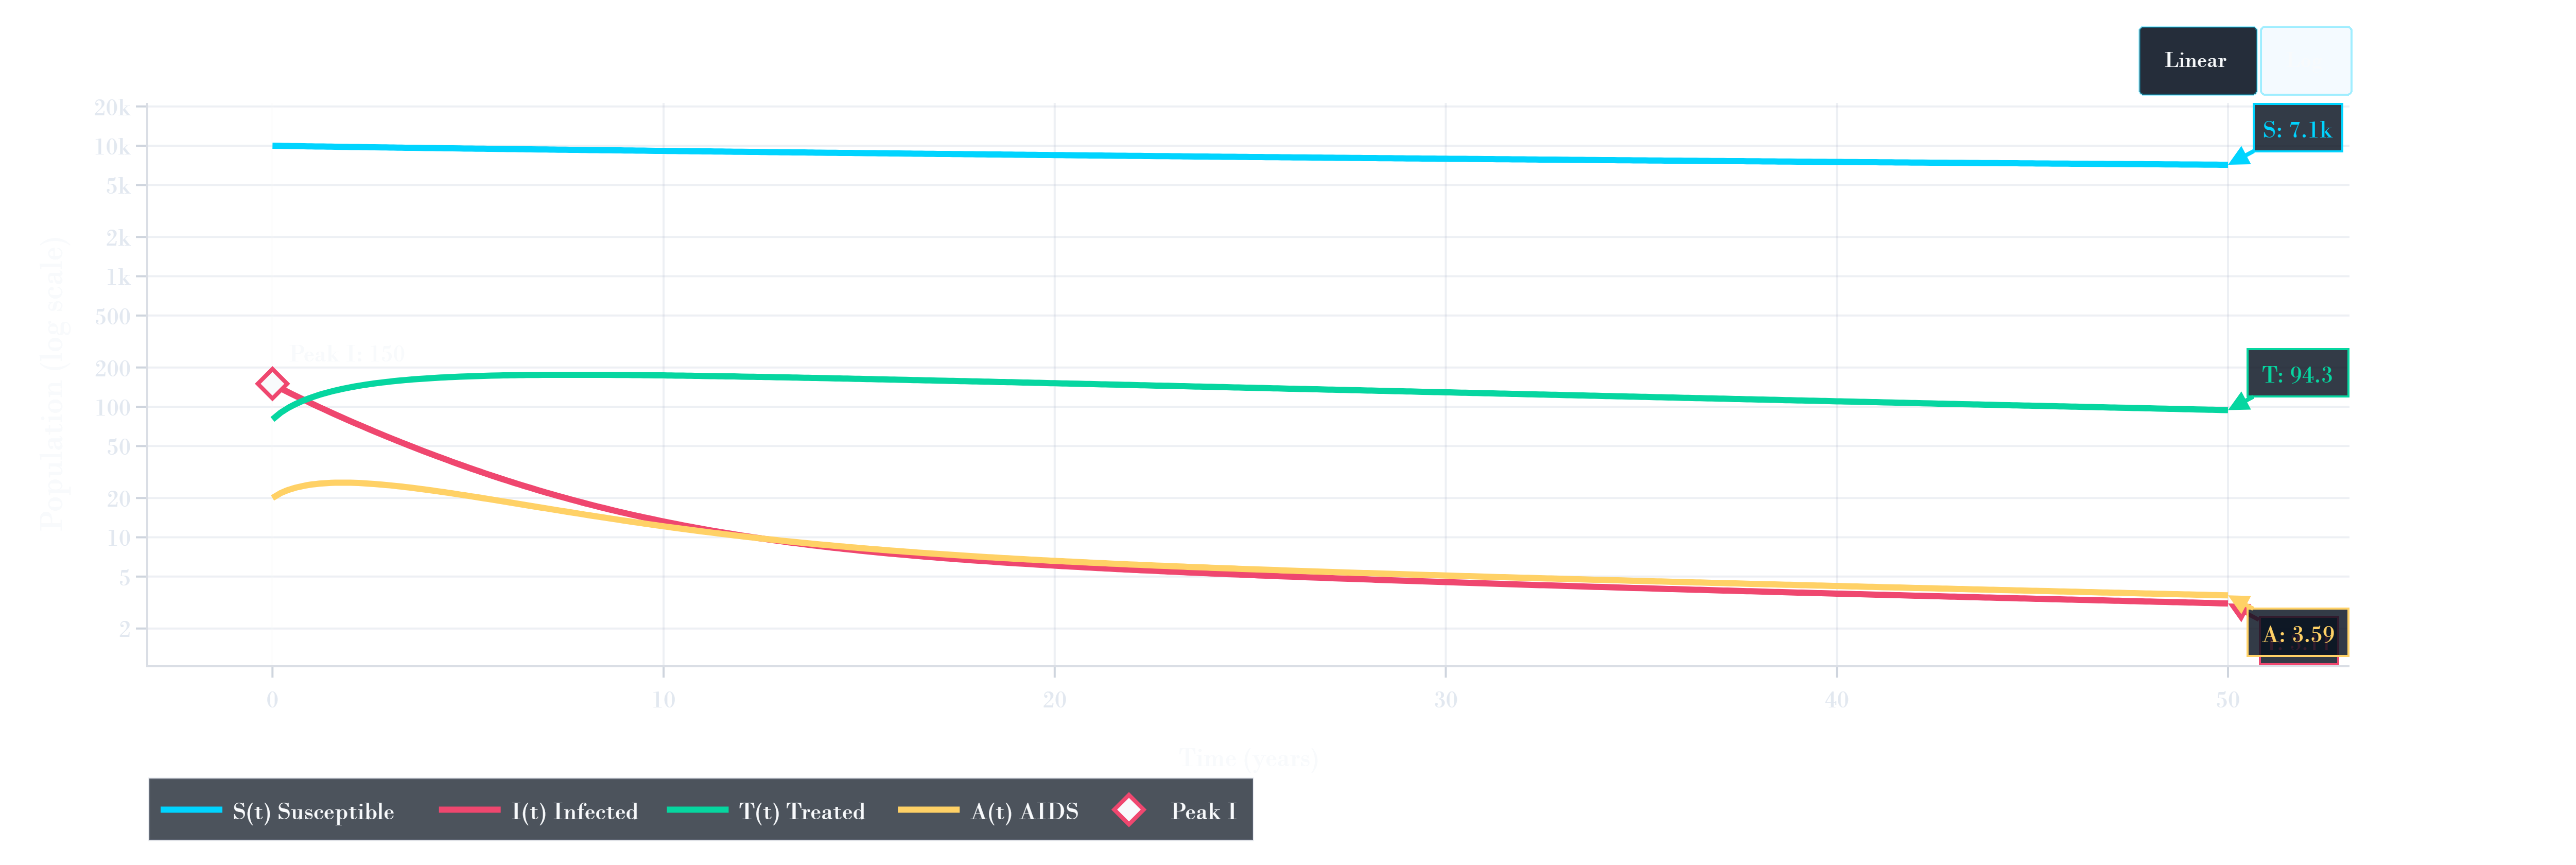
\includegraphics[width=\linewidth]{mainChartlinear.png}
\end{figureframe}
\caption{Baseline SITA time-series graph in the dashboard linear view.}
\label{fig:baseline_sita_linear}
\end{subfigure}

\vspace{0.4cm}

\begin{subfigure}{0.98\textwidth}
\centering
\begin{figureframe}[colframe=urblue, borderline west={3pt}{0pt}{urgold}]
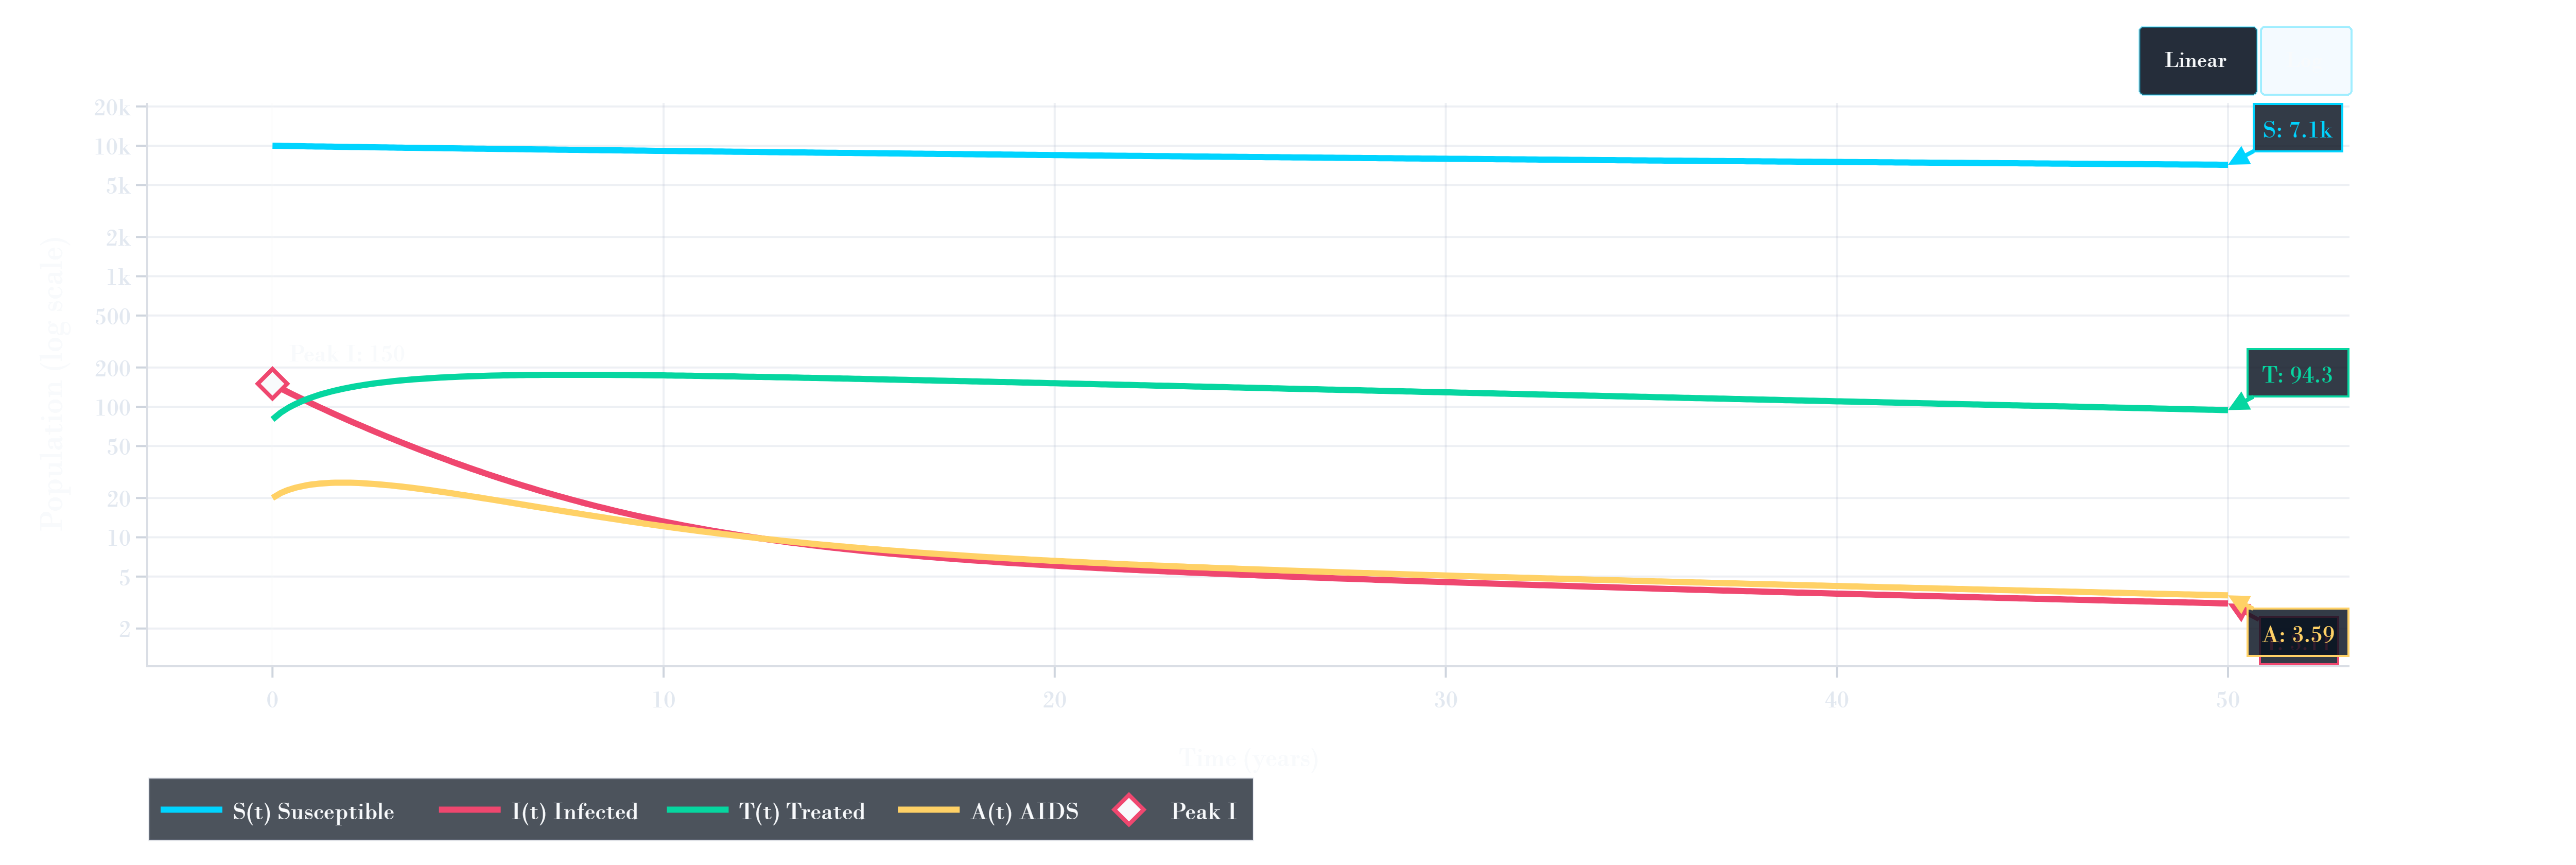
\includegraphics[width=\linewidth]{mainChartlog.png}
\end{figureframe}
\caption{Baseline SITA time-series graph in logarithmic view.}
\label{fig:baseline_sita_log}
\end{subfigure}
\caption{Baseline fractional-order SITA simulation for $q=0.95$ showing $S(t)$, $I(t)$, $T(t)$, and $A(t)$.}
\label{fig:baseline_sita_simulation}
\end{figure}

Figure~\ref{fig:baseline_sita_simulation} shows the baseline behaviour of the four model compartments. The susceptible population $S(t)$ remains the largest compartment throughout the simulation and decreases gradually from the initial value of 10000 to approximately 7146.82 at the final time. The infected population $I(t)$ starts at its highest value of 150 and then decreases continuously, reaching approximately 3.11 by year 50. This decline is consistent with the computed value $\mathcal{R}_0=0.430<1$, which indicates controlled transmission under the selected intervention levels.

The treated class $T(t)$ initially increases because infected individuals are moved into treatment through the testing and treatment-seeking intervention. After reaching a higher level, it gradually decreases and ends at approximately 94.27. The AIDS-stage class $A(t)$ remains low compared with the susceptible and treated compartments and ends at approximately 3.59. The logarithmic view is especially useful because it makes the smaller infected, treated, and AIDS-stage curves visible on the same graph as the much larger susceptible population.

\begin{table}[H]
\centering
\caption{Baseline simulation summary for the fractional SITA model.}
\label{tab:baseline_results}
\begin{tabular}{lcc}
\toprule
Quantity & Value & Interpretation\\
\midrule
$\mathcal{R}_0$ & 0.430 & Controlled epidemic status\\
Peak infected & 150.00 & Occurs at $t=0.0$ years\\
Final susceptible, $S(50)$ & 7146.82 & Susceptible population at final time\\
Final infected, $I(50)$ & 3.11 & Infected population at final time\\
Final treated, $T(50)$ & 94.27 & Treated population at final time\\
Final AIDS, $A(50)$ & 3.59 & AIDS-stage population at final time\\
\bottomrule
\end{tabular}
\end{table}

The baseline results show a strong decline in the infected class. The infected population starts at 150 individuals and decreases to approximately 3.11 individuals by the end of the simulation period. The treated class remains higher than the infected and AIDS classes at the final time, which is consistent with the effect of testing and treatment-seeking intervention. The AIDS-stage population also remains low, which reflects the effect of adherence support in reducing progression from treatment to AIDS.

\section{Effect of Fractional Order}
The fractional order $q$ controls the strength of memory in the Caputo fractional derivative. When $q=1$, the model reduces to the classical ordinary differential equation model. When $0<q<1$, the model contains memory effects, meaning that previous states of the system continue to influence the present dynamics through the fractional kernel.

To examine the role of memory, the model was simulated using four values of the fractional order:
\[
q=1.00,\qquad q=0.95,\qquad q=0.85,\qquad q=0.75.
\]
All other parameter values were kept fixed so that the differences in the trajectories could be attributed to the change in $q$.

\begin{figure}[H]
\centering
\begin{subfigure}{0.48\textwidth}
\centering
\begin{figureframe}[colframe=mathgreen, borderline west={3pt}{0pt}{urblue}]
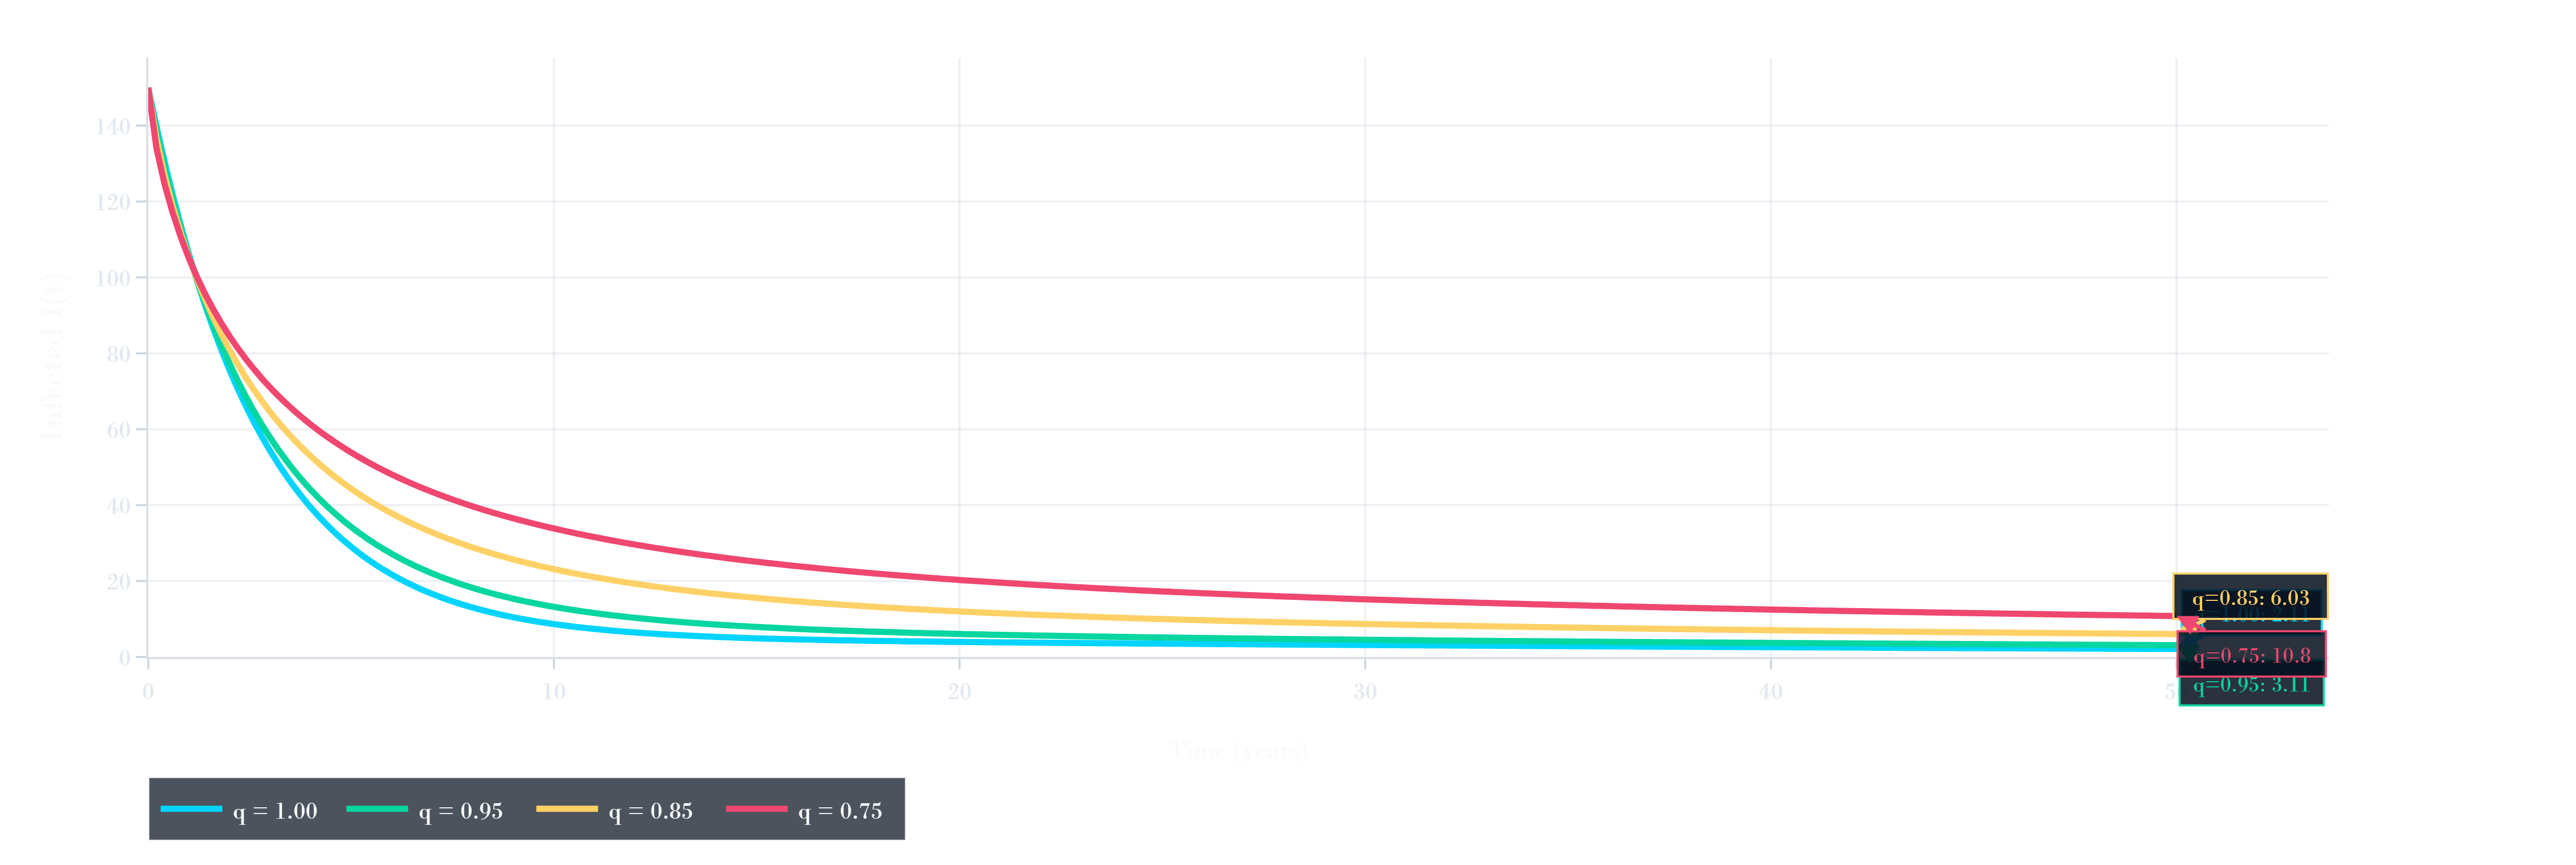
\includegraphics[width=\linewidth]{memoryChart.png}
\end{figureframe}
\caption{Infected population $I(t)$.}
\label{fig:memory_infected}
\end{subfigure}
\hfill
\begin{subfigure}{0.48\textwidth}
\centering
\begin{figureframe}[colframe=mathgreen, borderline west={3pt}{0pt}{urgold}]
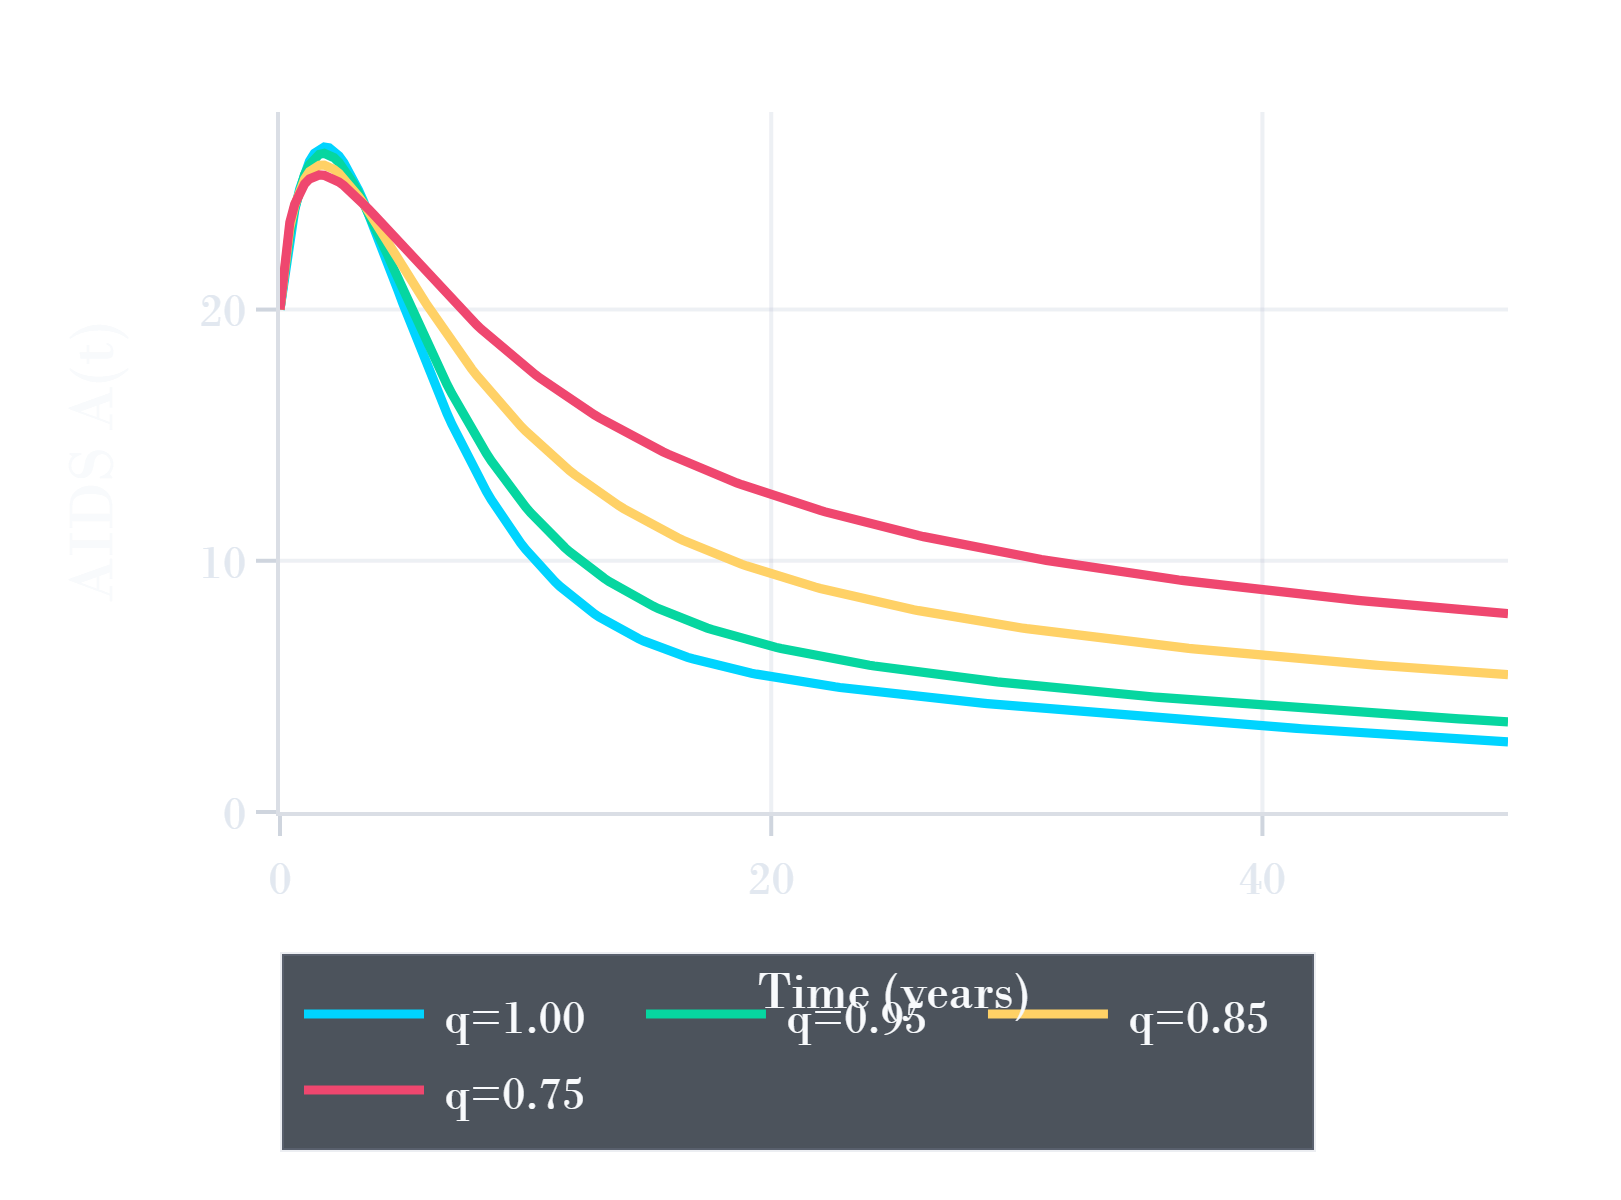
\includegraphics[width=\linewidth]{memoryAChart.png}
\end{figureframe}
\caption{AIDS-stage population $A(t)$.}
\label{fig:memory_aids}
\end{subfigure}

\vspace{0.25cm}

\begin{subfigure}{0.48\textwidth}
\centering
\begin{figureframe}[colframe=urblue, borderline west={3pt}{0pt}{mathgreen}]
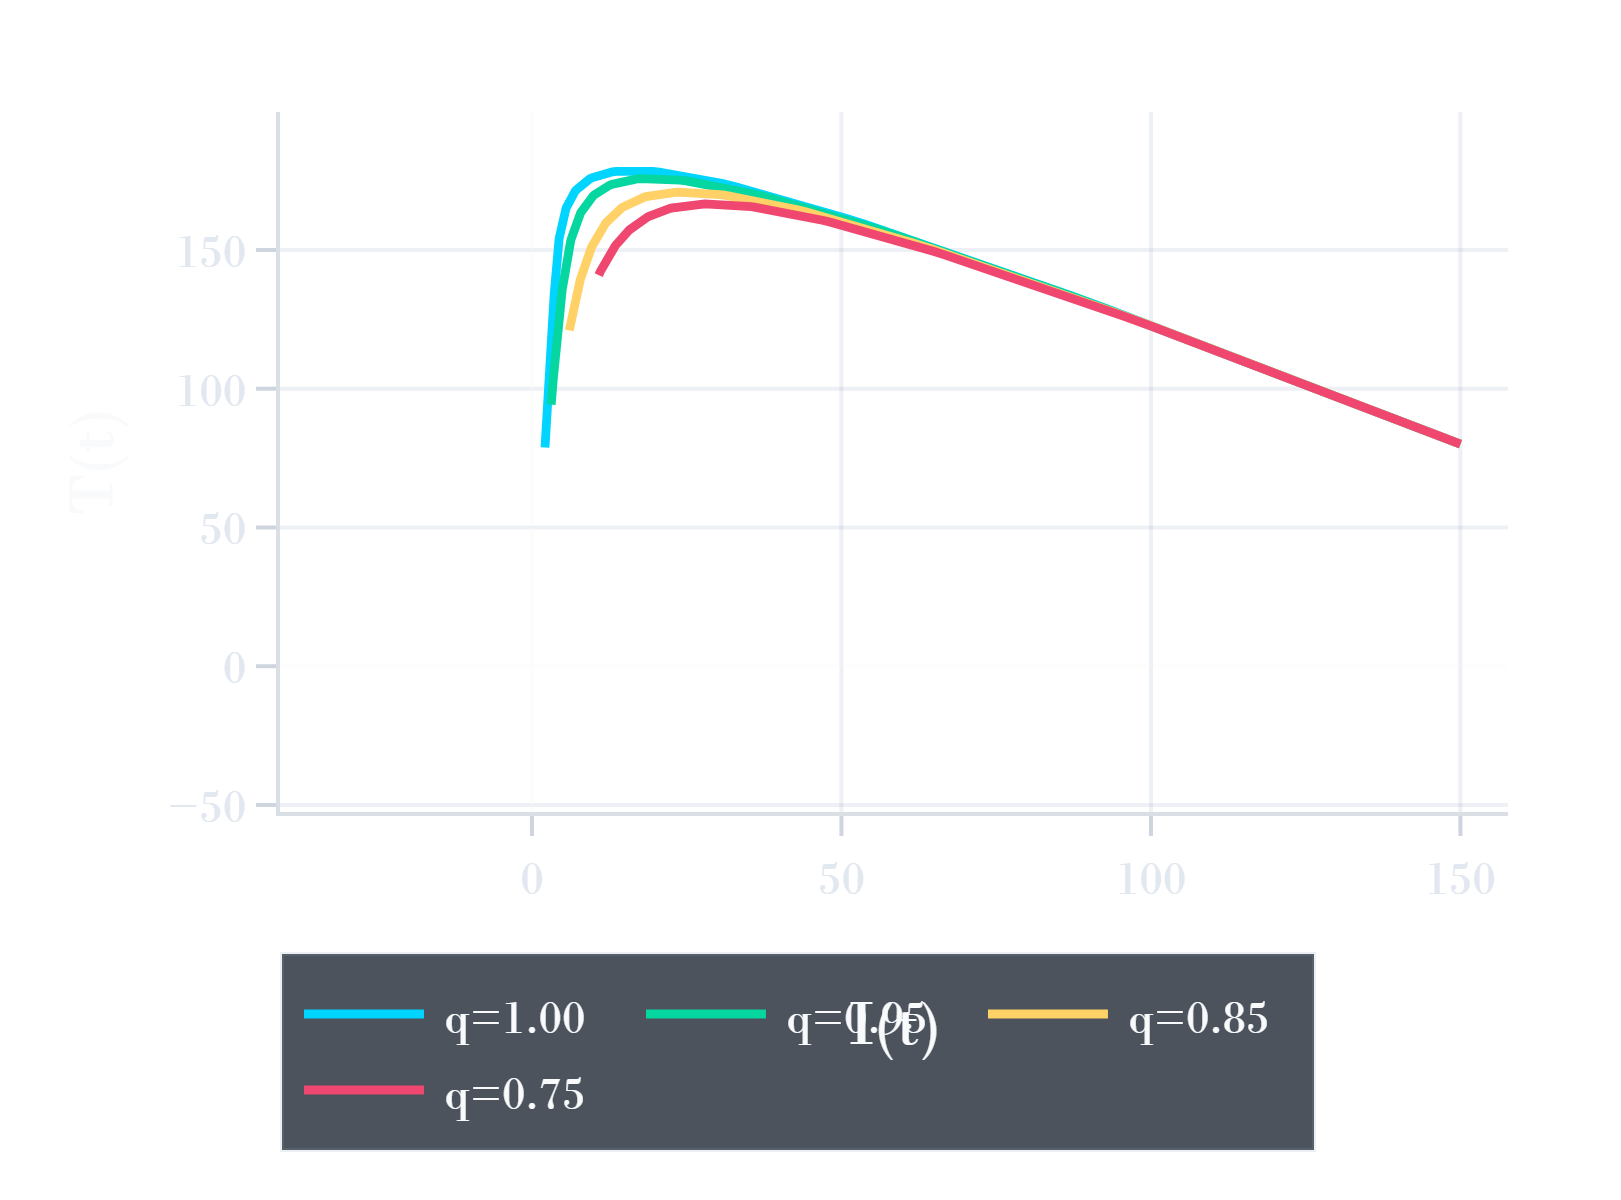
\includegraphics[width=\linewidth]{memoryPhaseChart.png}
\end{figureframe}
\caption{Phase trajectory in the $I$--$T$ plane.}
\label{fig:memory_phase}
\end{subfigure}
\hfill
\begin{subfigure}{0.48\textwidth}
\centering
\begin{figureframe}[colframe=brickred, borderline west={3pt}{0pt}{urblue}]
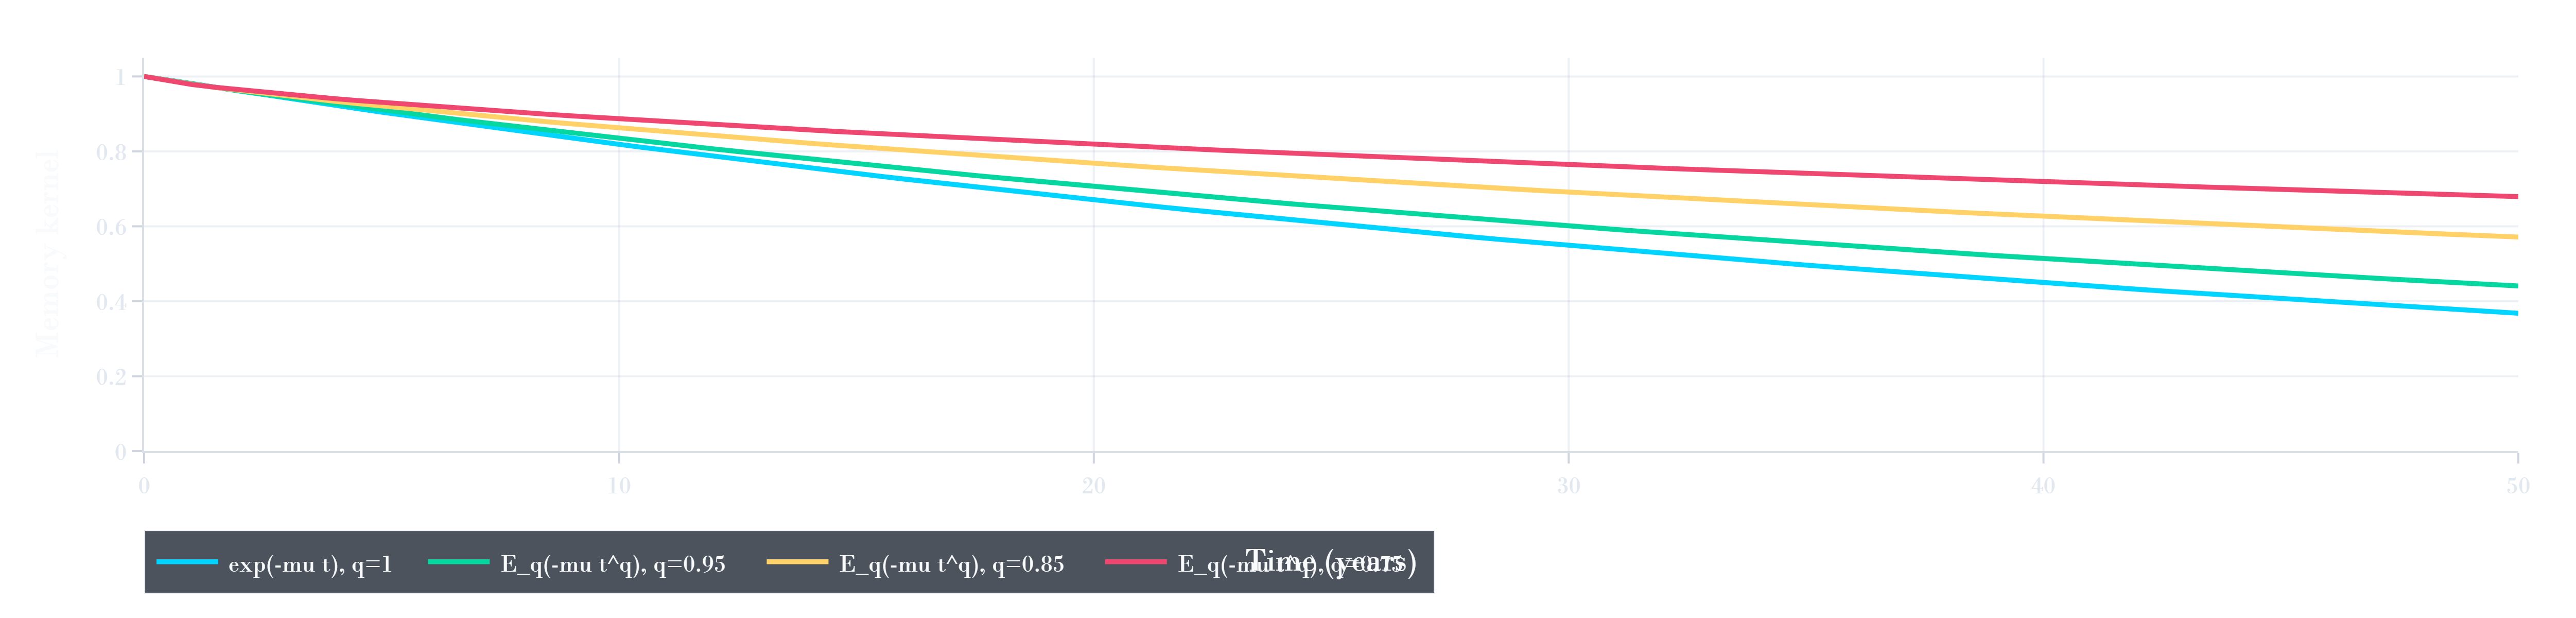
\includegraphics[width=\linewidth]{mittagChart.png}
\end{figureframe}
\caption{Mittag--Leffler memory kernel.}
\label{fig:mittag_kernel}
\end{subfigure}
\caption{Two-by-two memory-effect dashboard visualisation for $q=1.00$, $q=0.95$, $q=0.85$, and $q=0.75$.}
\label{fig:memory_extra}
\end{figure}

Figure~\ref{fig:memory_extra} compares the model response for $q=1.00$, $q=0.95$, $q=0.85$, and $q=0.75$ in a compact two-by-two layout. In Figure~\ref{fig:memory_infected}, all infected curves begin from the same initial value, but their decline rates are different. The ordinary model with $q=1.00$ decreases fastest, while the lower fractional order $q=0.75$ decreases slowest and remains highest at the final time. This confirms that stronger fractional memory delays the movement of the system toward the disease-free state.

In Figure~\ref{fig:memory_aids}, the AIDS-stage population first increases slightly and then decreases over time. The curve for the lower fractional order $q=0.75$ remains higher for longer, while the ordinary case $q=1.00$ decreases faster. This means that stronger memory effects can delay the reduction of the AIDS-stage population.

The phase graph in Figure~\ref{fig:memory_phase} shows the relationship between the infected and treated compartments. The trajectories move through a similar region of the phase plane, but the curves separate according to the fractional order. This indicates that changing $q$ affects not only the size of each compartment but also the dynamic relationship between infection and treatment.

Figure~\ref{fig:mittag_kernel} shows the fractional memory kernel. The ordinary exponential case decreases faster, while the Mittag--Leffler type curves associated with fractional orders decay more slowly. This supports the interpretation that fractional models preserve past effects for a longer period than classical ordinary differential equation models.

\begin{table}[H]
\centering
\caption{Comparison of simulation outcomes for different fractional orders.}
\label{tab:memory_results}
\begin{tabular}{cccccc}
\toprule
$q$ & Peak $I$ & Time of peak & Final $I$ & Final $T$ & Final $A$\\
\midrule
1.00 & 150.00 & 0.00 & 2.11 & 78.78 & 2.79\\
0.95 & 150.00 & 0.00 & 3.11 & 94.27 & 3.59\\
0.85 & 150.00 & 0.00 & 6.03 & 120.99 & 5.47\\
0.75 & 150.00 & 0.00 & 10.79 & 140.94 & 7.90\\
\bottomrule
\end{tabular}
\end{table}

The results show that decreasing the fractional order changes the long-term behaviour of the system. For $q=1.00$, the final infected population is approximately 2.11, while for $q=0.75$ it increases to approximately 10.79. Similarly, the treated and AIDS-stage populations are higher for smaller values of $q$. This indicates that stronger memory effects slow the rate at which the system approaches the controlled state. In epidemiological terms, this supports the idea that past behavioural patterns, treatment history, and adherence behaviour may continue to influence HIV dynamics over time.

\section{Effect of Single Interventions}
This section examines the effect of each intervention when applied separately. The purpose is to identify how awareness, safer sexual behaviour, testing and treatment-seeking, and adherence influence the model before they are combined. Four single-intervention scenarios were considered:
\[
\text{awareness only},\qquad
\text{safer behaviour only},\qquad
\text{testing only},\qquad
\text{adherence only}.
\]

\begin{figure}[H]
\centering
\begin{figureframe}[colframe=urblue, borderline west={3pt}{0pt}{urgold}]
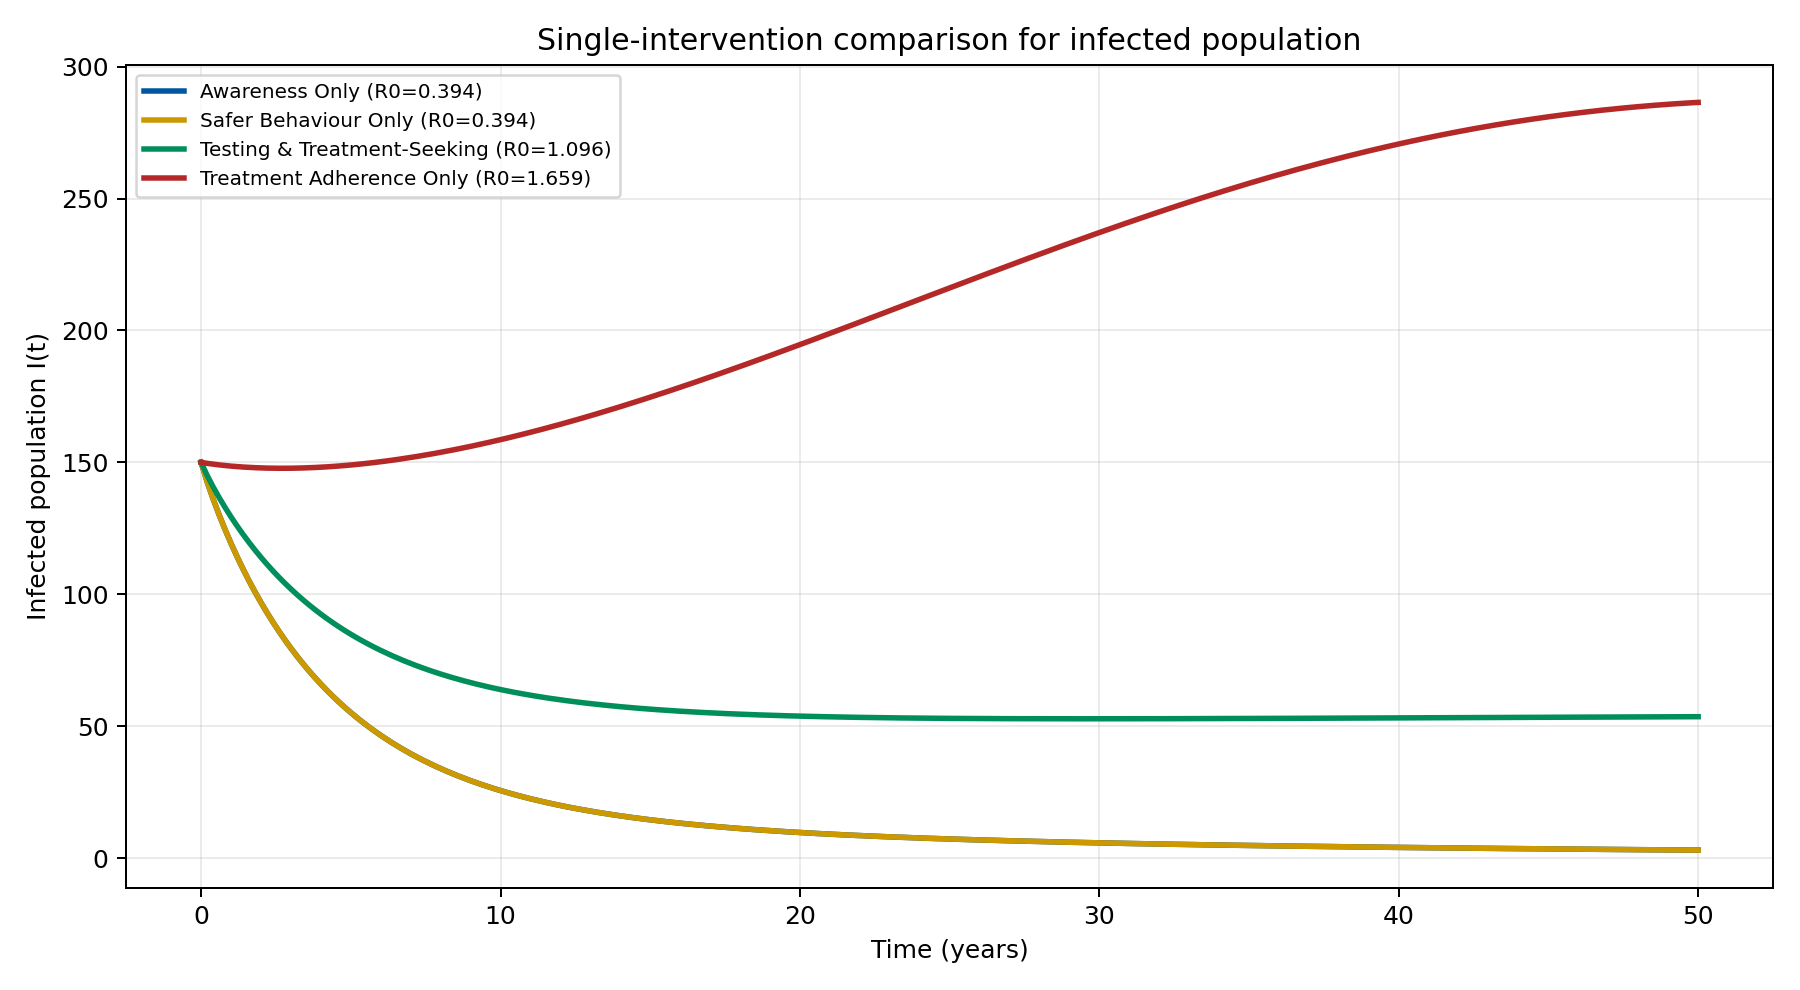
\includegraphics[width=0.94\textwidth]{singleInterventionsChart.png}
\end{figureframe}
\caption{Effect of single interventions on the infected population.}
\label{fig:single_interventions_infected}
\end{figure}

\begin{table}[H]
\centering
\caption{Single-intervention scenario results.}
\label{tab:single_interventions}
\begin{tabular}{lcccc}
\toprule
Scenario & $\mathcal{R}_0$ & Peak $I$ & Final $I$ & Final $A$\\
\midrule
Awareness only & 0.394 & 150.00 & 3.03 & 5.24\\
Safer behaviour only & 0.394 & 150.00 & 3.03 & 5.24\\
Testing and treatment-seeking & 1.096 & 150.00 & 53.60 & 43.90\\
Treatment adherence only & 1.659 & 286.44 & 286.44 & 99.45\\
\bottomrule
\end{tabular}
\end{table}

The awareness-only and safer-behaviour-only scenarios both reduce the effective transmission rate and give $\mathcal{R}_0=0.394$, which is below the epidemic threshold. This shows that interventions acting directly on transmission can strongly reduce the reproduction number. Testing and treatment-seeking alone improves movement from the infected class to the treated class, but it does not directly reduce transmission in the same way as awareness or safer behaviour. As a result, the reproduction number remains above one in the testing-only case. Adherence support alone reduces progression from treatment to AIDS, but it does not sufficiently reduce new infections when used in isolation; therefore, the model still shows persistence under that scenario.

These results show that single interventions can be useful, but their effectiveness depends on which model pathway they influence. Interventions that reduce transmission have a stronger direct effect on $\mathcal{R}_0$, while treatment-related interventions mainly influence the distribution between infected, treated, and AIDS-stage compartments.

\section{Combined Intervention Strategy}
The combined intervention strategy applies several forms of control at the same time. This is important because HIV transmission is not controlled by one factor only. Awareness, safer behaviour, testing, treatment access, and adherence all contribute to the long-term epidemic outcome.

Three combined scenarios were simulated: a moderate combined intervention, the main combined intervention, and a strong combined intervention. The results are shown in Table~\ref{tab:combined_interventions}.

\begin{figure}[H]
\centering
\begin{figureframe}[colframe=mathgreen, borderline west={3pt}{0pt}{urblue}]
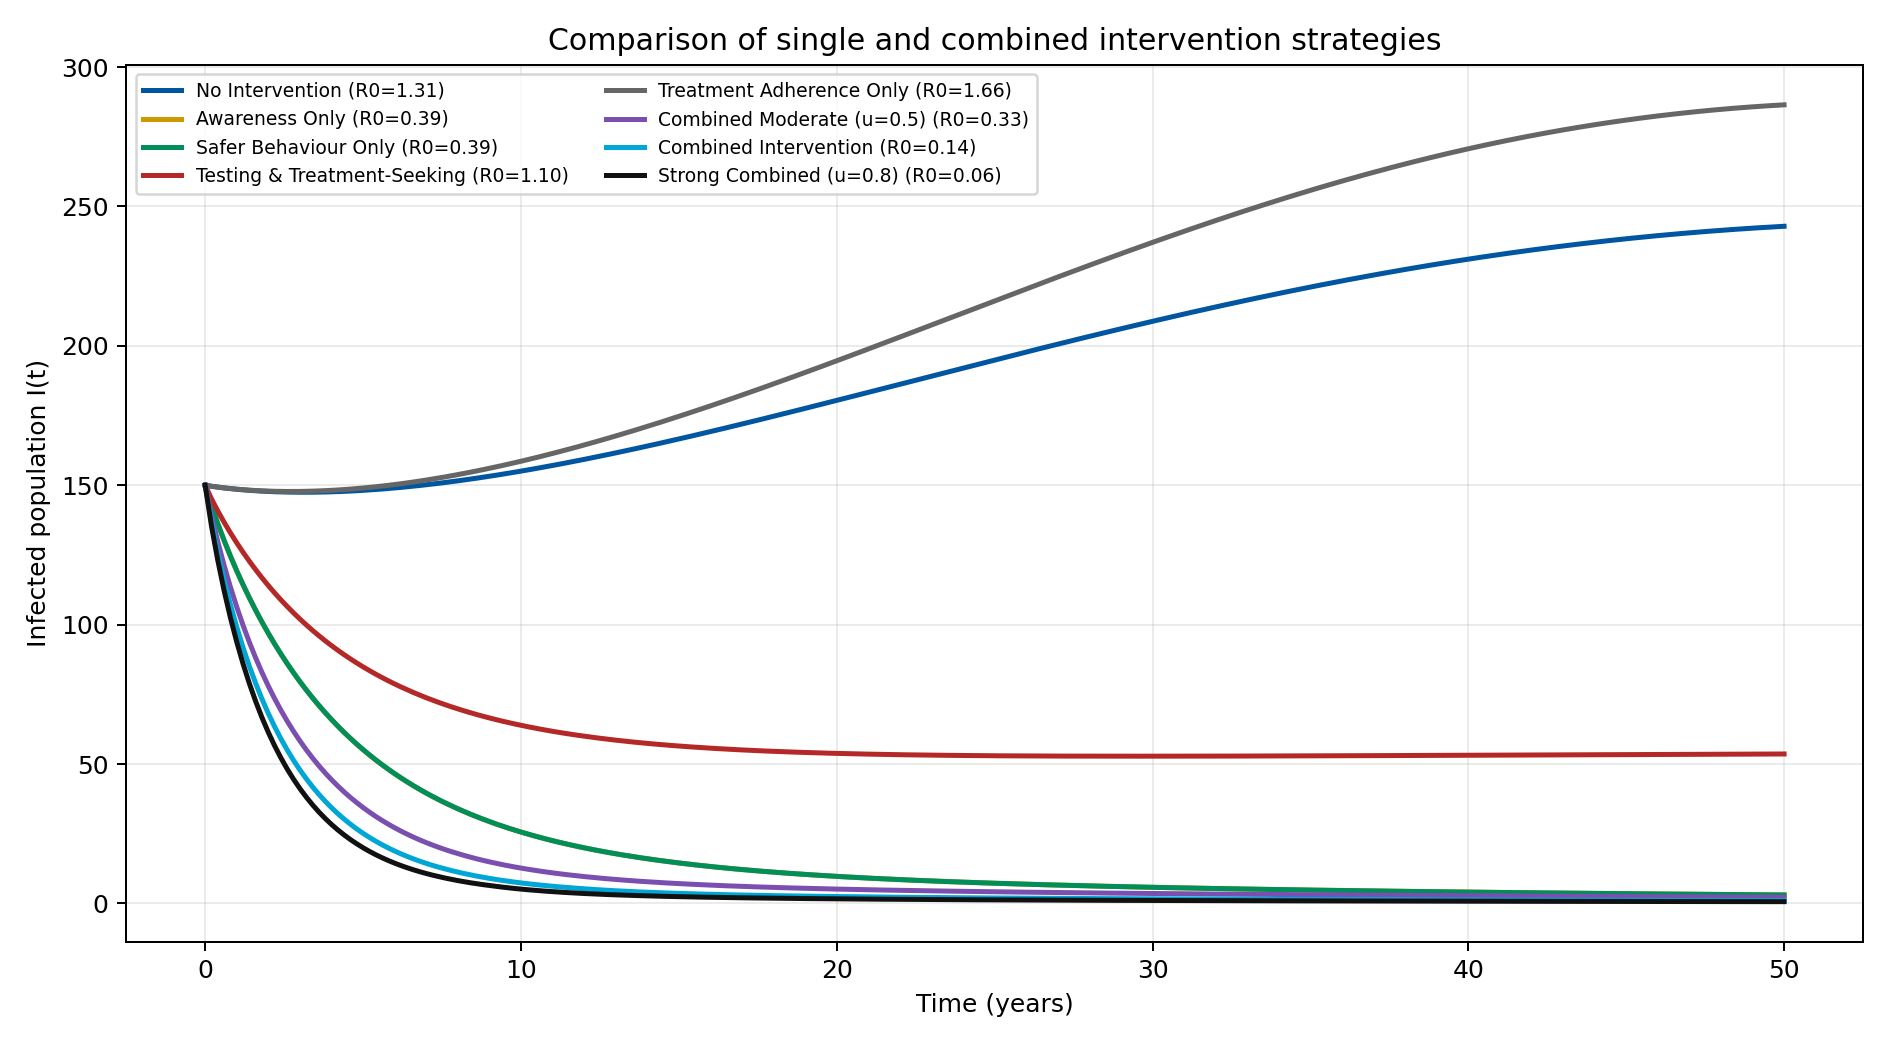
\includegraphics[width=0.94\textwidth]{combinedInterventionsChart.png}
\end{figureframe}
\caption{Comparison of single and combined intervention strategies.}
\label{fig:combined_intervention}
\end{figure}

\begin{table}[H]
\centering
\caption{Combined-intervention scenario results.}
\label{tab:combined_interventions}
\begin{tabular}{lcccc}
\toprule
Scenario & $\mathcal{R}_0$ & Peak $I$ & Final $I$ & Final $A$\\
\midrule
Combined intervention & 0.137 & 150.00 & 1.03 & 1.80\\
Combined moderate $(u=0.5)$ & 0.332 & 150.00 & 2.21 & 3.95\\
Strong combined $(u=0.8)$ & 0.060 & 150.00 & 0.64 & 1.61\\
\bottomrule
\end{tabular}
\end{table}

The combined intervention strategies produce the strongest control results. The main combined intervention gives $\mathcal{R}_0=0.137$, while the strong combined intervention gives $\mathcal{R}_0=0.060$. Both values are far below one, indicating strong epidemic control. The final infected population also decreases substantially, reaching approximately 1.03 under the main combined intervention and 0.64 under the strong combined intervention.

These results support the conclusion that combined interventions are more effective than isolated intervention strategies. In particular, reducing transmission while also improving testing, treatment uptake, and adherence produces better long-term control than focusing on one pathway alone.

\section{Sensitivity Analysis Results}
Sensitivity analysis was used to identify the parameters and intervention controls that have the strongest influence on the basic reproduction number. The normalized sensitivity index measures the proportional change in $\mathcal{R}_0$ caused by a proportional change in a parameter. A positive sensitivity index means that increasing the parameter increases $\mathcal{R}_0$, while a negative index means that increasing the parameter reduces $\mathcal{R}_0$.

\begin{figure}[H]
\centering
\begin{figureframe}[colframe=brickred, borderline west={3pt}{0pt}{urgold}]
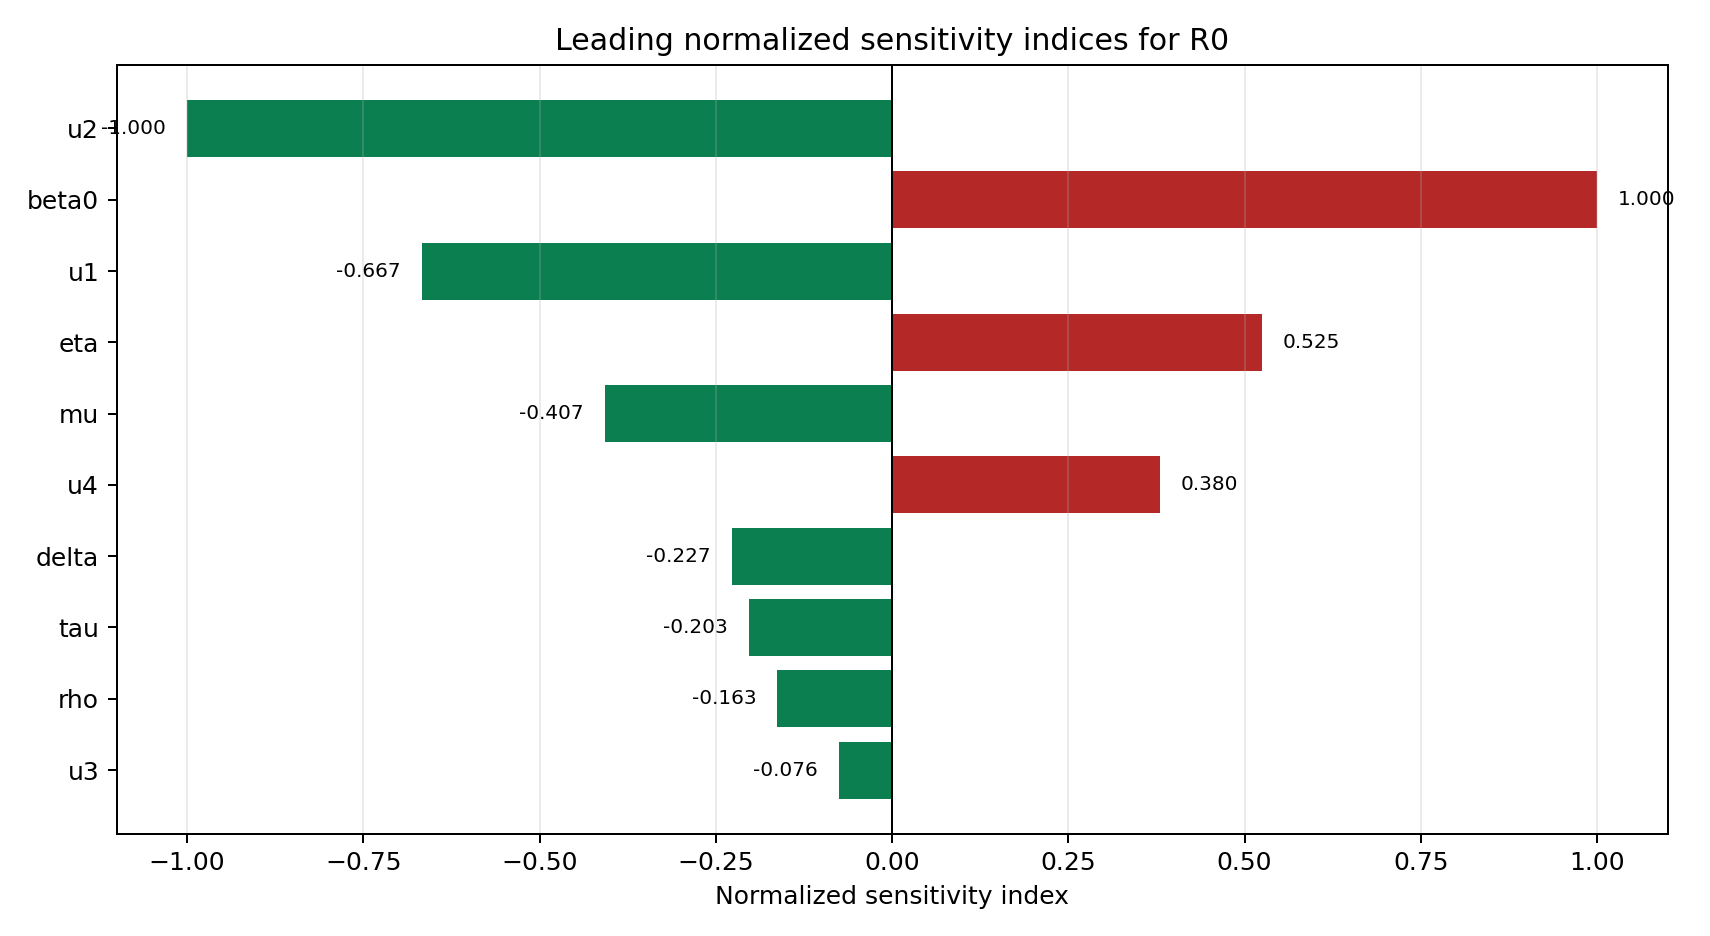
\includegraphics[width=0.90\textwidth]{sensitivityChart.png}
\end{figureframe}
\caption{Normalized sensitivity indices for $\mathcal{R}_0$.}
\label{fig:sensitivity_indices}
\end{figure}

\begin{table}[H]
\centering
\caption{Leading normalized sensitivity indices for $\mathcal{R}_0$.}
\label{tab:sensitivity_results}
\begin{tabular}{lc}
\toprule
Parameter or control & Sensitivity index\\
\midrule
$u_2$ & -1.000\\
$\beta_0$ & 1.000\\
$u_1$ & -0.667\\
$\eta$ & 0.525\\
$\mu$ & -0.407\\
$u_4$ & 0.380\\
$\delta$ & -0.227\\
$\tau$ & -0.203\\
\bottomrule
\end{tabular}
\end{table}

The baseline transmission rate $\beta_0$ has a positive sensitivity index of approximately 1.000, which means that increasing the baseline transmission rate increases $\mathcal{R}_0$ almost proportionally. The safer-behaviour intervention $u_2$ has a sensitivity index of approximately $-1.000$, showing that increasing safer behaviour strongly reduces $\mathcal{R}_0$. Awareness $u_1$ also has a negative sensitivity index, confirming its role in reducing effective transmission.

The sensitivity results therefore support the intervention findings: reducing transmission is central to controlling the epidemic threshold. Treatment and adherence parameters also affect the system, especially by changing movement into treatment and progression to AIDS, but transmission-related factors are the strongest drivers of $\mathcal{R}_0$ in this configuration.

\section{Dashboard Demonstration}
The computational part of this report was implemented as an interactive Flask dashboard. The dashboard allows the user to adjust initial conditions, biological parameters, fractional order, and intervention levels. It then displays time-series graphs, $\mathcal{R}_0$, stability interpretation, scenario comparison, memory-effect comparison, sensitivity analysis, and export tools.

\begin{figure}[H]
\centering
\begin{figureframe}[colframe=urblue, borderline west={3pt}{0pt}{urgold}]
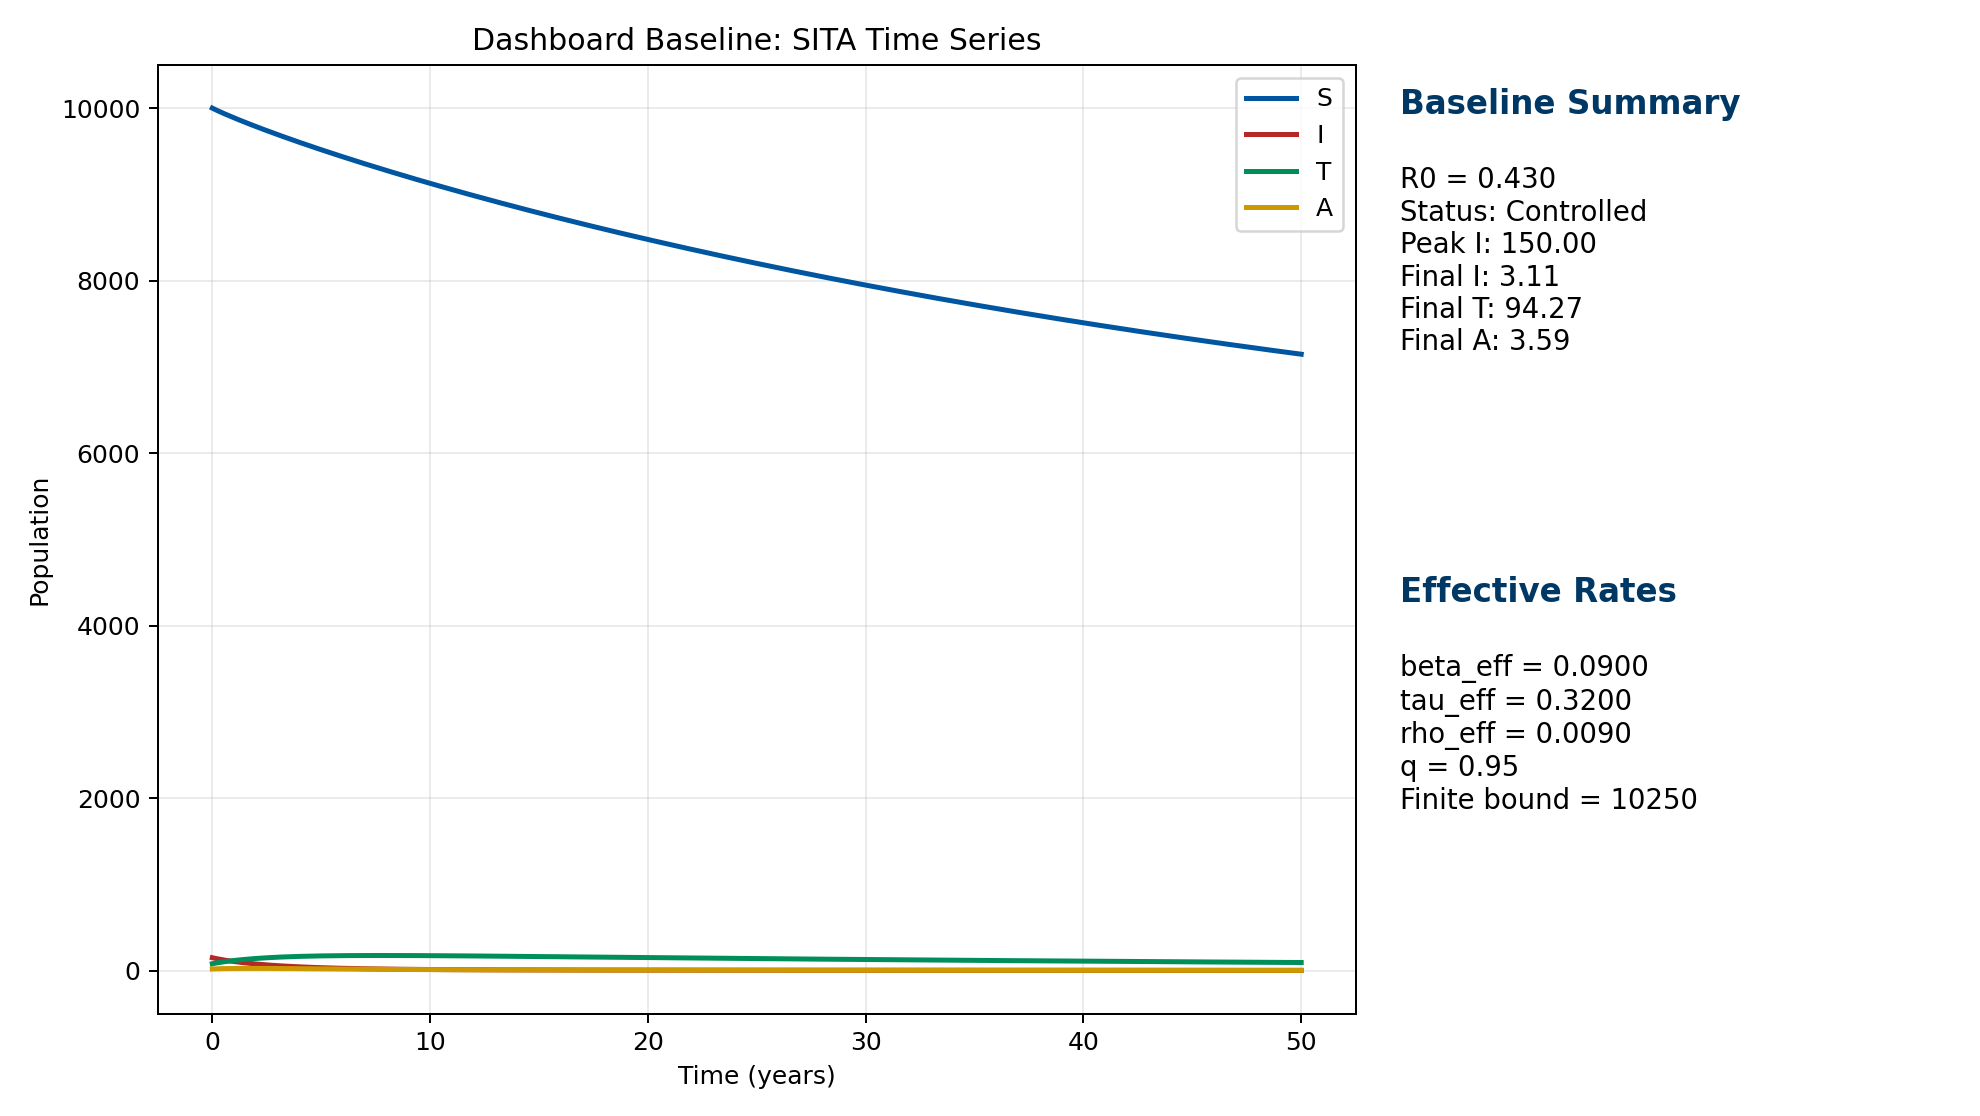
\includegraphics[width=0.94\textwidth]{dashboardBaselineFigure.png}
\end{figureframe}
\caption{Dashboard baseline simulation interface.}
\label{fig:dashboard_baseline}
\end{figure}

\begin{figure}[H]
\centering
\begin{figureframe}[colframe=mathgreen, borderline west={3pt}{0pt}{urblue}]
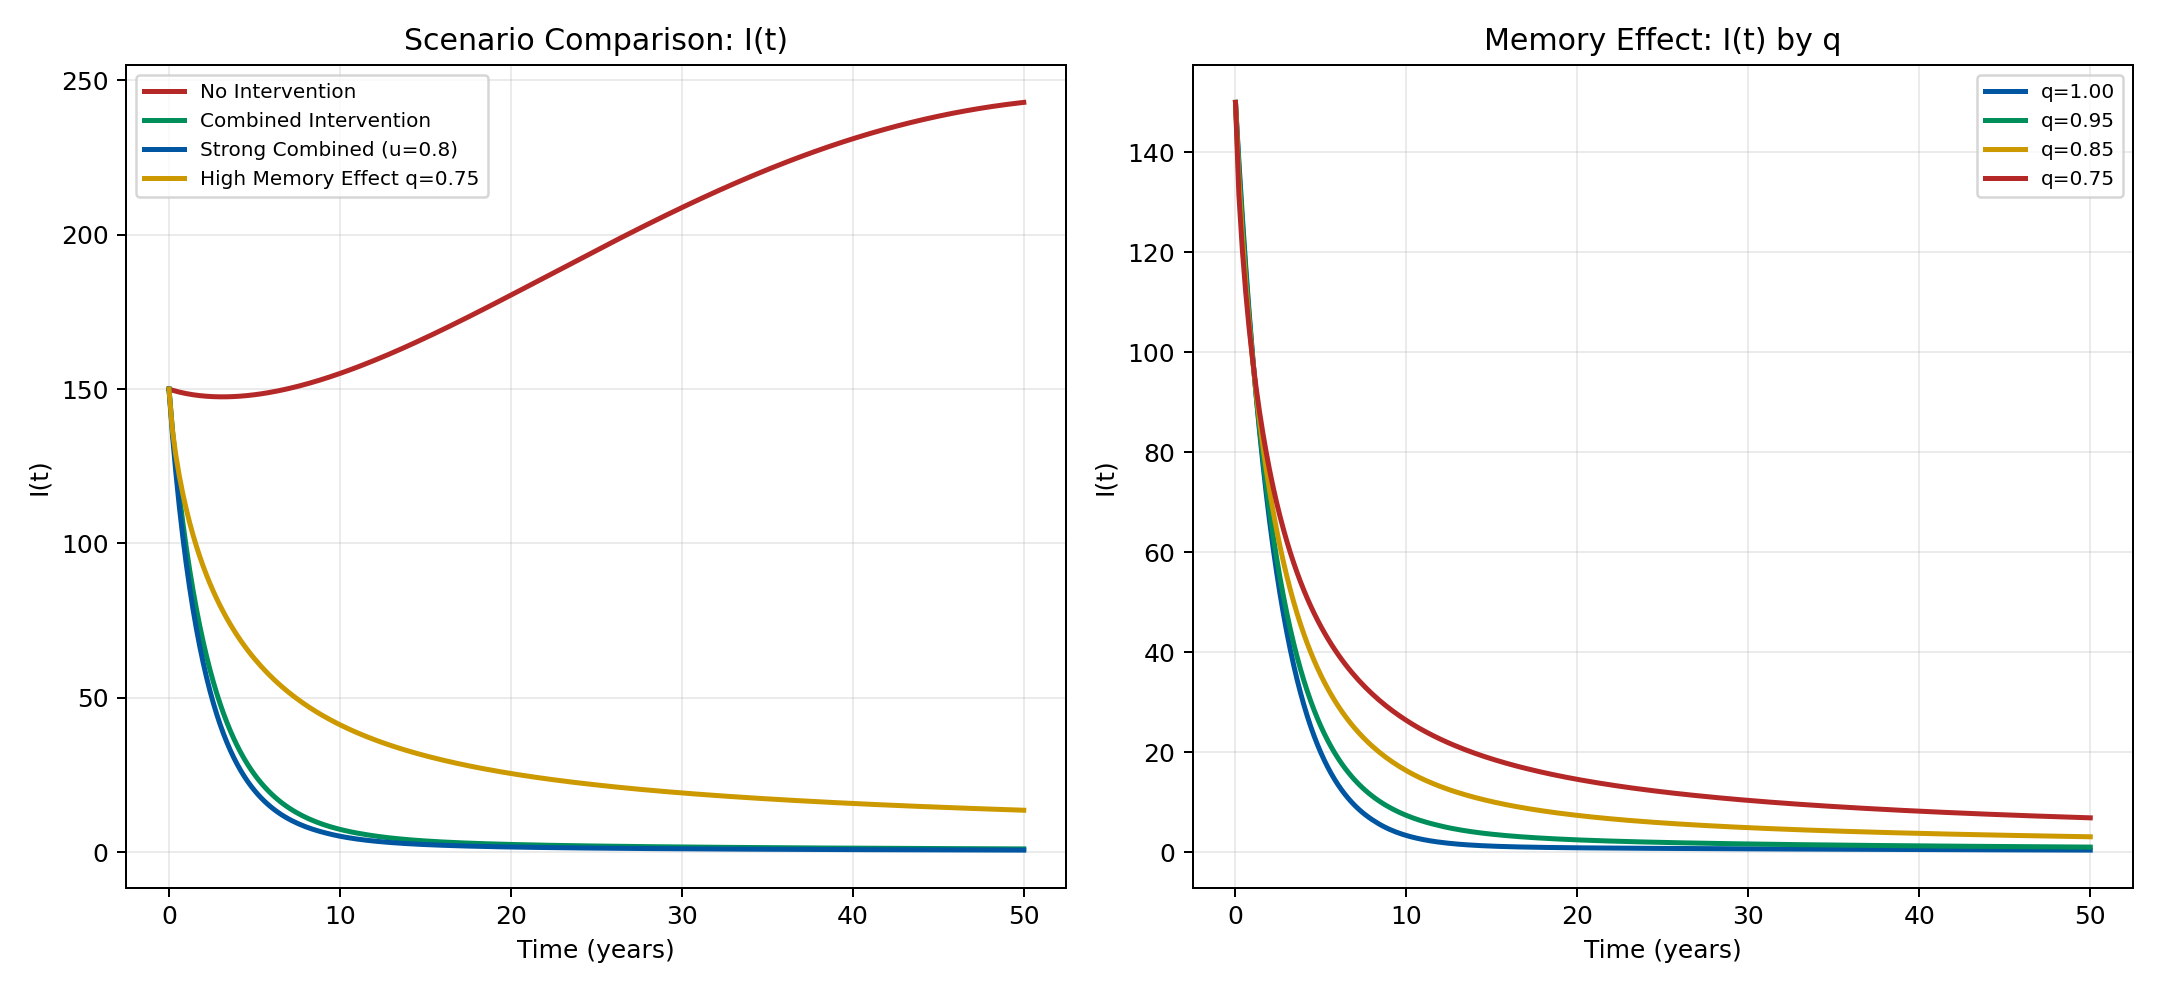
\includegraphics[width=0.94\textwidth]{dashboardScenarioMemoryFigure.png}
\end{figureframe}
\caption{Dashboard scenario and memory-effect visualisation.}
\label{fig:dashboard_scenarios_memory}
\end{figure}

\begin{figure}[H]
\centering
\begin{figureframe}[colframe=brickred, borderline west={3pt}{0pt}{urblue}]
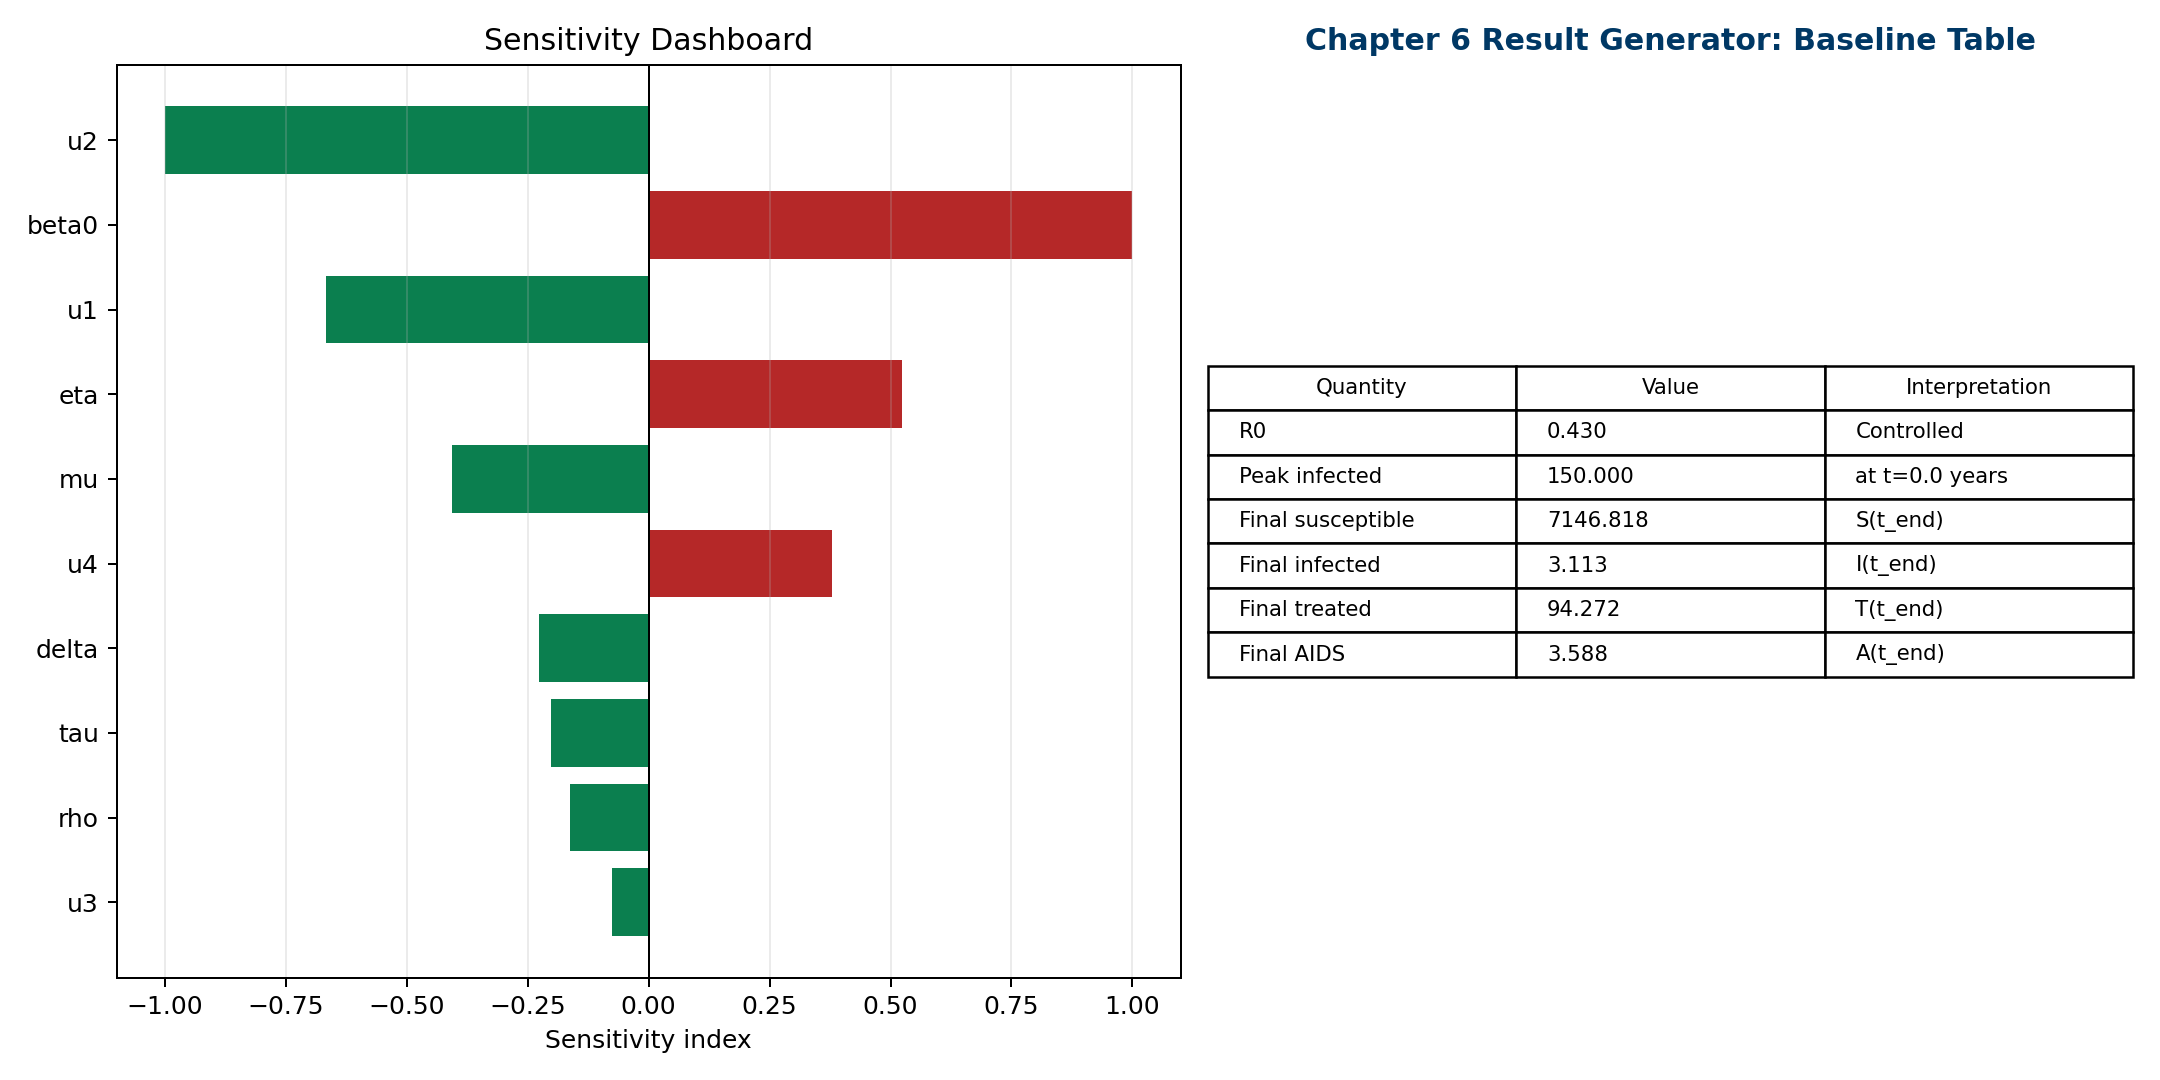
\includegraphics[width=0.94\textwidth]{dashboardSensitivityChapter6Figure.png}
\end{figureframe}
\caption{Dashboard sensitivity analysis and report-result generator.}
\label{fig:dashboard_sensitivity_chapter6}
\end{figure}

The dashboard supports the report in three main ways. First, it provides visual evidence for the analytical model by plotting the numerical trajectories of the four compartments. Second, it allows intervention scenarios to be compared using the same baseline parameter values. Third, it provides export tools for CSV tables, figures, and report-ready interpretation text. This makes the mathematical model easier to communicate during project writing and presentation.

\section{Public Health Interpretation}
The numerical results have direct public-health interpretation, although the model is intended for academic simulation rather than clinical prediction. The results show that interventions reducing effective transmission have a strong effect on the reproduction number. In practical terms, awareness campaigns, risk-reduction education, condom use, and safer sexual behaviour can reduce the probability that susceptible individuals become infected.

Testing and treatment-seeking interventions are also important because they move infected individuals into treatment more quickly. This reduces the untreated infected population and increases the treated population. Treatment adherence reduces progression from treatment to AIDS, helping to keep the AIDS-stage population lower. These findings are consistent with the idea that HIV control requires both prevention and treatment support.

In the context of Rwanda's HIV response, the model supports the importance of integrated intervention programmes. Rwanda has made progress in HIV testing, treatment, and viral suppression, but continued prevention and adherence support remain important. The combined-intervention simulations show that applying behavioural and biomedical interventions together produces stronger control than applying one intervention alone.

The fractional-order results also provide an important interpretation. When $q<1$, past behaviour and treatment history influence present dynamics through memory effects. This reflects the fact that public health interventions may not act instantaneously; instead, their influence may persist over time through community awareness, adherence habits, stigma reduction, and accumulated treatment experience.

%% ============================================================
\chapter{Conclusion and Recommendations}
%% ============================================================

\section{Conclusion}
This report develops a fractional-order SITA HIV transmission model incorporating social behaviour interventions. The use of Caputo fractional derivatives allows the model to capture memory effects, while the Gamma and Mittag-Leffler functions provide the mathematical foundation for the fractional framework. The model connects HIV transmission, treatment initiation, AIDS progression, and behavioural interventions in a single mathematical structure.

The theoretical analysis focuses on positivity, boundedness, disease-free equilibrium, the basic reproduction number, and fractional-order stability. The computational component demonstrates how fractional dynamics and social behaviour interventions can be explored through simulation and dashboard visualisation.

\section{Recommendations}
\begin{enumerate}
  \item Future work may include age or gender structure.
  \item Future studies may estimate parameters using Rwanda-specific data.
  \item Stochastic fractional models may be considered for small populations.
  \item The dashboard may be extended into a decision-support educational tool.
  \item Other fractional operators, such as Caputo--Fabrizio or Atangana--Baleanu derivatives, may be compared with the Caputo derivative.
\end{enumerate}

\section{Limitations of the Study}
\begin{enumerate}
  \item The model assumes homogeneous mixing.
  \item Parameter values are literature-informed and scaled for scenario comparison, but they are not fitted to patient-level Rwanda data.
  \item The model is deterministic and does not include random effects.
  \item The intervention functions simplify complex human behaviour into bounded mathematical controls.
  \item The dashboard is for academic simulation, not clinical prediction.
\end{enumerate}

%% REFERENCES
%% ============================================================
\begin{thebibliography}{99}
\addcontentsline{toc}{chapter}{References}

\bibitem[Anderson and May(1991)]{AndersonMay1991}
Anderson, R. M., and May, R. M. (1991).
\textit{Infectious Diseases of Humans: Dynamics and Control}.
Oxford University Press.

\bibitem[Caputo(1967)]{Caputo1967}
Caputo, M. (1967).
Linear models of dissipation whose Q is almost frequency independent.
\textit{Geophysical Journal International}, 13(5), 529--539.

\bibitem[Diethelm et al.(2002)]{Diethelm2002}
Diethelm, K., Ford, N. J., and Freed, A. D. (2002).
A predictor-corrector approach for the numerical solution of fractional differential equations.
\textit{Nonlinear Dynamics}, 29, 3--22.

\bibitem[Diethelm(2010)]{Diethelm2010}
Diethelm, K. (2010).
\textit{The Analysis of Fractional Differential Equations}.
Springer.

\bibitem[Diekmann et al.(1990)]{Diekmann1990}
Diekmann, O., Heesterbeek, J. A. P., and Metz, J. A. J. (1990).
On the definition and the computation of the basic reproduction ratio $R_0$ in models for infectious diseases in heterogeneous populations.
\textit{Journal of Mathematical Biology}, 28, 365--382.

\bibitem[Günerhan et al.(2020)]{Gunerhan2020}
Günerhan, H., Dutta, H., Dokuyucu, M. A., and Adel, W. (2020).
Analysis of a fractional HIV model with Caputo and constant proportional Caputo operators.
\textit{Chaos, Solitons \& Fractals}, 139, 110053.
\url{https://doi.org/10.1016/j.chaos.2020.110053}

\bibitem[Hethcote(2000)]{Hethcote2000}
Hethcote, H. W. (2000).
The mathematics of infectious diseases.
\textit{SIAM Review}, 42(4), 599--653.

\bibitem[Kermack and McKendrick(1927)]{Kermack1927}
Kermack, W. O., and McKendrick, A. G. (1927).
A contribution to the mathematical theory of epidemics.
\textit{Proceedings of the Royal Society A}, 115(772), 700--721.

\bibitem[Kilbas et al.(2006)]{Kilbas2006}
Kilbas, A. A., Srivastava, H. M., and Trujillo, J. J. (2006).
\textit{Theory and Applications of Fractional Differential Equations}.
Elsevier.

\bibitem[Matignon(1996)]{Matignon1996}
Matignon, D. (1996).
Stability results for fractional differential equations with applications to control processing.
\textit{Computational Engineering in Systems Applications}, 2, 963--968.

\bibitem[Podlubny(1999)]{Podlubny1999}
Podlubny, I. (1999).
\textit{Fractional Differential Equations}.
Academic Press.

\bibitem[Poundstone et al.(2004)]{Poundstone2004}
Poundstone, K. E., Strathdee, S. A., and Celentano, D. D. (2004).
The social epidemiology of human immunodeficiency virus/acquired immunodeficiency syndrome.
\textit{Epidemiologic Reviews}, 26(1), 22--35.
\url{https://doi.org/10.1093/epirev/mxh005}

\bibitem[RBC(2020)]{RBC2020RPHIA}
Rwanda Biomedical Centre. (2020).
\textit{Rwanda Population-Based HIV Impact Assessment (RPHIA) 2018--2019: Final Report}.
Kigali: Rwanda Biomedical Centre.
\url{https://phia.icap.columbia.edu/rwanda-final-report/}

\bibitem[RRP+(2020)]{RRP2020Stigma}
Rwanda Network of People Living with HIV (RRP+). (2020).
\textit{Rwanda: People Living with HIV Stigma Index 2.0 Survey Report}.
\url{https://rrpplus.org/rwanda-people-living-with-hiv-index-2-0-survey-report-2020/}

\bibitem[Silva and Torres(2017)]{SilvaTorres2017}
Silva, C. J., and Torres, D. F. M. (2017).
A SICA compartmental model in epidemiology with application to HIV/AIDS in Cape Verde.
\textit{Ecological Complexity}, 30, 70--75.

\bibitem[Supervie et al.(2011)]{Supervie2011}
Supervie, V., Barrett, M., Kahn, J. S., Musuka, G., Moeti, T. L., Busang, L., et al. (2011).
Modeling dynamic interactions between pre-exposure prophylaxis interventions and treatment programs: predicting HIV transmission and resistance.
\textit{Scientific Reports}, 1, 185.
\url{https://doi.org/10.1038/srep00185}

\bibitem[UNAIDS(2025)]{UNAIDS2025FactSheet}
UNAIDS. (2025).
\textit{Global HIV \& AIDS Statistics — Fact Sheet}.
\url{https://www.unaids.org/en/resources/fact-sheet}

\bibitem[Unaegbu et al.(2021)]{Unaegbu2021}
Unaegbu, E. N., et al. (2021).
A fractional order HIV/AIDS model using Caputo-Fabrizio operator.
\textit{African Journal of Infectious Diseases}, 15(2 Suppl.), 1--18.
\url{https://doi.org/10.21010/Ajid.v15i2S.1}

\bibitem[Van den Driessche and Watmough(2002)]{VanDenDriessche2002}
Van den Driessche, P., and Watmough, J. (2002).
Reproduction numbers and sub-threshold endemic equilibria for compartmental models of disease transmission.
\textit{Mathematical Biosciences}, 180(1--2), 29--48.

\bibitem[WHO(2025)]{WHO2025HIV}
World Health Organization. (2025).
\textit{HIV and AIDS Fact Sheet}.
\url{https://www.who.int/news-room/fact-sheets/detail/hiv-aids}

\end{thebibliography}

\clearpage
%% ============================================================
%% APPENDICES
%% ============================================================
\appendix
\chapter*{Appendices}
\addcontentsline{toc}{chapter}{Appendices}
\markboth{Appendices}{Appendices}

\begin{remarkbox}[title={Purpose of the Appendices}]
The appendices provide supporting implementation material for the fractional-order HIV dashboard. They are placed after the References in accordance with the recommended final thesis structure. The material is supplementary: it supports reproducibility and documentation, while the main mathematical formulation, analysis, and results remain in the body of the report.
\end{remarkbox}

\chapter{Dashboard Implementation Support}

\section{Project Folder Structure}
The following structure summarises the organisation of the Python dashboard used to implement the fractional-order SITA model, run simulations, expose API routes, and export figures or reports.

\begin{lstlisting}[
  style=pythonstyle,
  basicstyle=\ttfamily\scriptsize,
  aboveskip=3pt,
  belowskip=3pt,
  lineskip=-1pt
]
fractional_hiv_project_dashboard/
|
|-- app.py
|-- config.py
|-- requirements.txt
|-- README.md
|
|-- model/
|   |-- fractional_sita_model.py
|   |-- fractional_solver.py
|   |-- reproduction_number.py
|   |-- scenarios.py
|   |-- sensitivity.py
|   `-- validation.py
|
|-- routes/
|   |-- simulation_routes.py
|   |-- export_routes.py
|   `-- health_routes.py
|
|-- templates/
|   |-- base.html
|   |-- index.html
|   |-- dashboard.html
|   |-- documentation.html
|   `-- about.html
|
|-- static/
|   |-- css/
|   |-- js/
|   |-- assets/
|   `-- vendor/
|
|-- data/
|   |-- baseline_parameters.json
|   |-- scenario_presets.json
|   `-- sample_outputs.csv
|
`-- outputs/
    |-- csv/
    |-- figures/
    `-- reports/
\end{lstlisting}

\section{Fractional ABM Solver Skeleton}
The following code skeleton shows the numerical idea behind the fractional Adams--Bashforth--Moulton predictor-corrector scheme used by the dashboard. The production implementation includes validation and dashboard-specific data formatting, while the skeleton below highlights the solver logic.

\begin{lstlisting}[
  style=pythonstyle,
  basicstyle=\ttfamily\scriptsize,
  aboveskip=3pt,
  belowskip=3pt,
  lineskip=-1pt
]
import numpy as np
from scipy.special import gamma

def fractional_abm_solver(rhs, y0, t, q, params):
    n = len(t)
    h = t[1] - t[0]
    y = np.zeros((n, len(y0)), dtype=float)
    y[0] = np.maximum(y0, 0.0)
    fvals = np.zeros_like(y)
    fvals[0] = rhs(t[0], y[0], params)

    for k in range(1, n):
        history = np.arange(k, 0, -1, dtype=float)
        b = history**q - (history - 1.0)**q
        y_pred = y[0] + (h**q / gamma(q + 1.0)) * (b @ fvals[:k])

        a = np.empty(k, dtype=float)
        a[0] = (k - 1)**(q + 1) - (k - 1 - q) * k**q
        if k > 1:
            m = np.arange(k - 1, 0, -1, dtype=float)
            a[1:] = (m + 1.0)**(q + 1) + (m - 1.0)**(q + 1) - 2.0*m**(q + 1)

        y[k] = y[0] + (h**q / gamma(q + 2.0)) * (
            rhs(t[k], y_pred, params) + (a @ fvals[:k])
        )
        y[k] = np.maximum(y[k], 0.0)
        fvals[k] = rhs(t[k], y[k], params)

    return y
\end{lstlisting}

\chapter{Supplementary Parameter Documentation}

\section{Baseline Parameter Summary}
Table~\ref{tab:appendix_parameter_summary} records the main model parameters used in the dashboard. The table is included as supplementary documentation to clarify how the computational interface relates to the mathematical notation in the report.

\begin{table}[H]
\centering
\small
\renewcommand{\arraystretch}{1.15}
\caption{Supplementary summary of baseline model parameters.}
\label{tab:appendix_parameter_summary}
\begin{tabular}{>{\bfseries}c p{6.5cm}p{3cm}}
\toprule
Parameter & Description & Baseline Status\\
\midrule
$\beta_0$ & Baseline transmission rate & Literature-guided\\
$\mu$ & Natural death rate & Demographic context\\
$\tau$ & Treatment initiation rate & Literature-guided\\
$\delta$ & Progression from infected to AIDS & Literature-guided\\
$\rho$ & Progression from treated to AIDS & Literature-guided\\
$d$ & AIDS-induced mortality & Literature-guided\\
$\eta$ & Relative infectiousness under treatment & Literature-guided\\
$q$ & Fractional order & Simulation parameter\\
$u_1,u_2,u_3,u_4$ & Social behaviour interventions & User-defined\\
\bottomrule
\end{tabular}
\end{table}

\end{document}
